\documentclass[11pt]{article}
\usepackage{packages/packages}
\usepackage{packages/macros}

\title{Lecture Notes: Basics of ML}
\author{Scott Pesme \\ \small INRIA Grenoble}
% \date{\today}

\begin{document}
\maketitle
\tableofcontents

\newpage

\section{Introduction}
Slides of the general introduction can be found \href{https://kernel-learning.github.io/docs/intro.pdf}{here}.


\section{Learning framework}

Before diving into any algorithm, let us informally describe what we mean by
\emph{learning} from data. The guiding idea of machine learning is to replace
explicit, hand-written rules by a procedure that \emph{extracts patterns from
examples}. Rather than telling a computer exactly how to recognise a cat, or how
to price a flat, we provide it with a collection of \emph{data} and let it
\emph{learn} a rule that performs well and, crucially, keeps performing
well on new data it has never seen. This section sets up the vocabulary; the
precise definitions and the mathematics come in the following sections.

\subsection{What is ``data''?}

Everything starts from \emph{data}: a collection of examples
$x_1, \dots, x_n$, where $n$ is the number of samples. Throughout these notes we
represent each example as a vector (sometimes called ``sample'' or ``input'') $x_i$, but this vector can encode
essentially anything, provided we agree on a way to turn the raw object into
numbers. A few concrete cases:
\begin{itemize}
    \item \emph{Feature vectors.} The most direct case, where each coordinate is
    an interpretable measurement. To describe a flat, one might take
    \[
    x = \big( [\text{surface in m}^2],\ [\text{number of rooms}],\ [\text{floor}],\ \dots \big) .
    \]
    \item \emph{Images.} A colour image of $H \times W$ pixels is a grid of RGB
    intensities. Flattening it gives a vector $x \in \R^d$ with $d = 3 H W$ (one
    coordinate per colour channel and pixel). A modest $224 \times 224$ image
    already lives in dimension $d \approx 1.5 \times 10^5$.
    \item \emph{Sound.} An audio clip is an amplitude sampled through time. If we
    record $d$ amplitudes, the clip is a vector $x \in \R^d$, one coordinate per time step.
    \item \emph{Text, graphs, \dots} Similarly, a piece of text, a molecule, or a
    social network can all be encoded as vectors once we fix a suitable
    representation.
\end{itemize}
The common thread is that, after a suitable encoding, every input becomes a
point $x_i \in \R^d$. This is what lets a single mathematical framework cover
such different-looking objects.

In \emph{supervised} problems each input $x_i$ comes with a \emph{label} $y_i$,
and the nature of $y$ varies just as much. It may be a real number
$y \in \R$ (a price, a temperature), a binary label $y \in \{0, 1\}$ (spam or
not), one of several categories $y \in \{1, \dots, K\}$ (which digit is written),
or even a structured object such as another image or a sentence. The two basic
regimes, real-valued and categorical labels, are exactly the regression and
classification problems we distinguish below.

\subsection{Supervised vs.\ unsupervised learning}

The first thing to ask about a learning problem is \emph{what the data looks
like}. This largely determines which family of methods is relevant.

\paragraph{Supervised learning.}
Here each data point comes as a \emph{pair} $(x, y)$: an \emph{input} (or
feature vector) $x$ together with a \emph{label} (or response) $y$ that we would
like to predict. The training set is a list
\[
(x_1, y_1), \dots, (x_n, y_n),
\]
and the goal is to learn a function $f$ such that $f(x) \approx y$, so that we
can predict the label of a \emph{new} input. The name ``supervised'' reflects
the fact that, for every training input, a supervisor has provided the correct
answer $y$. Predicting the price of a flat from its characteristics, or deciding
whether an email is spam, are typical examples.

\paragraph{Unsupervised learning.}
Now the data consists of \emph{inputs only},
\[
x_1, \dots, x_n,
\]
with no labels attached. Since there is nothing specific to predict, the goal
shifts to \emph{discovering structure} in the data on its own. Typical tasks
include \emph{clustering} (grouping similar points together) and \emph{dimensionality
reduction} (finding a few directions that capture most of the variability). We will see these in \Cref{sec:unsupervised}, through the $K$-means algorithm and principal component
analysis respectively.

\paragraph{Self-supervised learning.}
A particularly powerful idea, and the engine behind most modern large-scale
models, is to \emph{manufacture the labels from the unlabelled data itself}.
In \emph{self-supervised} learning one starts from inputs only and creates an
artificial supervised problem by hiding part
of each data point and asking the model to predict it from the rest. No human
annotation is required, yet the resulting task looks supervised. The typical
example is language modelling: take a sentence, hide a word (or simply ask for
the next one), and predict it from its surrounding context; repeating this over
enormous text corpora is how large language models are trained. The same recipe
applies to images (predict missing patches) or audio. Having learned rich
representations this way, the model can then be adapted to an actual downstream
task using comparatively few labels.

\begin{remark}[Other paradigms]
Supervised and unsupervised learning are the two pillars of this course, but
they do not exhaust machine learning. In \emph{reinforcement learning}, for
instance, an agent interacts with an environment and learns from \emph{rewards}
rather than from labelled examples: think of a program learning to play a
game by trial and error. We will not treat it here.
\end{remark}

\subsection{Supervised learning: regression vs.\ classification}

Within supervised learning, problems are further split according to the
\emph{nature of the label} $y$ we want to predict.

\paragraph{Regression.}
When the label is a \emph{real-valued} (continuous) quantity, $y \in \R$, we
speak of a \emph{regression} problem. Predicting a price, a temperature, or a
person's age from a photograph are regression tasks. This is the setting we
develop in detail in the next section.

\paragraph{Classification.}
When the label takes its values in a \emph{finite set of categories}, we speak
of a \emph{classification} problem. With two categories,
$y \in \{0, 1\}$ (or $\{-1, +1\}$), the problem is called \emph{binary}
classification, e.g.\ spam vs.\ not spam, healthy vs.\ sick. With more than
two categories, $y \in \{1, \dots, K\}$, it is \emph{multi-class}, e.g.\
recognising which digit, from $0$ to $9$, is written in an image.

\begin{remark}[Same recipe, different label]
Regression and classification share the very same blueprint: a class of
candidate functions, a way to measure the quality of a prediction, and an
algorithm that searches for a good function. What changes is mostly the type of
$y$ and, consequently, the loss used to compare a prediction with the truth.
Mastering regression therefore gives us most of the tools needed for
classification as well.
\end{remark}


\newpage
\section{Regression}
\label{sec:regression}

\subsection{The regression problem}

In a \emph{regression} problem we want to predict a real-valued quantity from
some input. The input is described by a \emph{feature vector}
$x \in \X \subseteq \R^d$, and the quantity we want to predict is a
\emph{response} $y \in \R$.

\begin{example}
Suppose we want to predict the price of a flat. Each flat can be encoded by a
feature vector
\[
x = \big( [\text{surface in m}^2],\ [\text{number of rooms}],\ [\text{floor}],\ \dots \big) \in \R^d ,
\]
and the response $y \in \R$ is its price. Each coordinate of $x$ is a
\emph{feature} (also called \emph{covariate} or \emph{explanatory variable}),
and $d$ is the number of features.
\end{example}

We are given a \emph{training set} of $n$ pairs
\[
(x_1, y_1), \dots, (x_n, y_n) \in \R^d \times \R ,
\]
where $n$ is the number of training samples and $d$ the dimension of each data
point. As in the rest of these notes, we stack the inputs into the
\emph{design matrix} and the outputs into a single vector:
\[
X = \begin{pmatrix}
- & x_1 & - \\
  & \vdots &  \\
- & x_n & -
\end{pmatrix} \in \R^{n \times d},
\qquad
y = (y_1, \dots, y_n) \in \R^n .
\]

\begin{remark}[Encoding non-numerical features]
We have implicitly assumed that each input is a vector of real numbers,
$x \in \R^d$. In practice many features are \emph{categorical} rather than
continuous: a person's sex (\texttt{male}/\texttt{female}), a colour, a city,
etc. We turn them into numbers as follows.
\begin{itemize}
    \item A \emph{binary} feature can be encoded by a single $-1/1$ indicator, e.g.\
    $\texttt{male} \mapsto -1$ and $\texttt{female} \mapsto 1$.
    \item A categorical feature with $K \geq 3$ possible values should
    \emph{not} simply be mapped to $1, 2, \dots, K$: this would invent a
    spurious order and notion of distance between categories (it would suggest
    that ``city $3$'' lies between ``city $2$'' and ``city $4$''). Instead one
    uses \emph{one-hot} (or \emph{dummy}) encoding: the feature is replaced by
    $K$ binary features, exactly one of which equals $1$. For example the colour
    $\{\texttt{red}, \texttt{green}, \texttt{blue}\}$ becomes
    \[
    \texttt{red} \mapsto (1,0,0), \quad
    \texttt{green} \mapsto (0,1,0), \quad
    \texttt{blue} \mapsto (0,0,1) .
    \]
    One might object that for $K = 2$ the one-hot encoding does not give back the "$-1/1$"
    encoding of the previous item. It in fact does; as explained later in the notes.
\end{itemize}
After such an encoding every input is again a genuine vector $x \in \R^d$, and
the whole framework below applies unchanged.
\end{remark}

The goal is to \emph{learn} a function $f : \X \to \R$ such that
\[
f(x) \approx y \qquad \text{for unseen pairs } (x, y).
\]
Once such an $f$ is found, we can predict the response of a brand new input
$x$ simply by evaluating $f(x)$.

\paragraph{What do we need to specify?}
Turning the vague wish ``$f(x) \approx y$'' into a well-posed problem requires
two ingredients:
\begin{enumerate}
    \item a \emph{class of functions} $\F$ in which we look for $f$ (e.g.\ all
    linear functions of $x$);
    \item a way to \emph{quantify} how good a candidate $f$ is on the data,
    i.e.\ a \emph{loss function}.
\end{enumerate}

\subsection{Choosing the function class}
\label{subsec:function-class}

The function class $\F$ collects all the candidate predictors we are willing to
consider. In practice we never search over an abstract set of functions:
instead we fix a \emph{parametrisation}, that is, we describe every candidate by
a finite vector of \emph{parameters} (or \emph{weights}) $w \in\R^p$ (where $p$ corresponds to the number of trainable parameters) and denote
the corresponding predictor by $f_w$. The function class is then
\[
\F = \big\{\, f_w \ : \ w \in \R^p \,\big\},
\]
and \emph{learning the function reduces to searching for a good parameter}
$w$.  How $w$ enters $f_w$ is a modelling choice; here are the main examples. (For
the linear models that occupy the rest of these notes the parameter has exactly one
coordinate per feature, so it lives in the same $\R^d$ as the inputs; the last two
examples below are parametrised differently, and there $w$ simply collects however
many weights the model has.)

\paragraph{Linear in the input.}
The simplest choice makes the prediction a linear function of the input,
\[
f_w(x) = \langle w, x \rangle = \sum_{j=1}^d w_j x_j , \qquad w \in \R^d ,
\]
so that the parameter $w$ has the same dimension $d$ as the input $x$ (i.e., $p = d$).


\paragraph{Nonlinear in the parameters.}
Nothing forces $w$ to enter linearly. One may equally consider parametrisations
in which the parameter appears \emph{inside} a nonlinear function: the resulting objective is non-convex in $w$, and must be tackled by
iterative optimisation (e.g.\ gradient descent), with no guarantee of reaching a
global minimum. The most prominent examples are neural networks.

\paragraph{Neural networks.}
A prominent and very expressive parametrisation that is nonlinear in $w$ is a
\emph{neural network}. In its simplest, one-hidden-layer form,
\[
f_w(x) = \sum_{k=1}^m a_k \, \sigma\big( \langle b_k, x\rangle + c_k \big),
\]
where $\sigma$ is a fixed nonlinearity (e.g.\ a ReLU or a sigmoid) and the
parameters $w = (a_k, b_k, c_k)_{k=1}^m$ gather all the weights. Increasing the
width $m$ (or stacking several such layers) yields an extremely rich
function class. The price to pay is, once more, a highly non-convex dependence
on $w$, which is the central difficulty of modern deep learning. 


\subsection{Choosing the loss function}

Fixing a function class is not enough: we still need to say what it means for a
prediction to be \emph{good}. This is the role of a \emph{loss function}
$\ell(\hat{y}, y)$, which quantifies how much we penalise predicting
$\hat{y} = f(x)$ when the true response is $y$. Averaging the loss over the
training set gives the \emph{empirical risk}, which we view as a function of the
parameter $w$ and denote
\[
L(w) = \frac{1}{n} \sum_{i=1}^n \ell\big( f_w(x_i), y_i \big).
\]
\emph{Empirical risk minimisation} then consists in choosing the parameter $w$
(equivalently, $f_w \in \F$) so as to make $L(w)$ as small as possible.

\begin{remark}[The constant $1/n$ does not matter for the minimiser]
Multiplying an objective by a positive constant does not move its minimisers:
for any $c > 0$, $\argmin_w c\, L(w) = \argmin_w L(w)$.
In particular the factor $1/n$ in front of the sum is immaterial when our only
goal is to \emph{locate} the best $w$. We nonetheless keep it throughout these
notes, because it makes $L(w)$ an \emph{average} loss per sample rather than a
total: its scale then does not grow with the size of the training set, and losses
computed on datasets of different sizes remain comparable. Be aware, though, that
the constant \emph{does} rescale the gradient $\nabla L$, and hence matters once a
step size enters the picture, as in gradient descent below. (The extra $\tfrac12$
that will appear for the squared error is a separate matter: it belongs to the
loss $\ell$ itself and is there only to cancel the $2$ coming from the derivative.)
\end{remark}

\paragraph{Several ways to penalise an error.}
The choice of $\ell$ is itself a modelling decision: different losses encode
different ideas of what a good fit is. A few common choices are
\begin{itemize}
    \item the \emph{squared error} $\ell(\hat{y}, y) = \tfrac{1}{2}(\hat{y} - y)^2$,
    by far the most common, which strongly penalises large residuals;
    \item the \emph{absolute error} $\ell(\hat{y}, y) = |\hat{y} - y|$, more
    robust to outliers but non-differentiable at~$0$;
    \item the \emph{Huber loss}, a compromise that is quadratic for small
    residuals and linear for large ones.
\end{itemize}
In the remainder of this section we focus on the squared error, which, when
combined with a model that is linear in $w$, yields the particularly clean
\emph{least-squares} problem.

\begin{remark}[Training error is not the goal]
Making the empirical risk small only guarantees that $f$ fits the
\emph{training} data. What we actually care about is the \emph{test error},
i.e.\ how well $f$ predicts on new, unseen inputs. A function can fit the
training set perfectly and still generalise poorly.
\end{remark}


\subsection{Minimising the empirical risk}

Choosing a function class and a loss has turned learning into an optimisation
problem:
\[
w^\star \in \argmin_{w \in \R^p} \ L(w),
\]
where $\argmin_w L(w)$ denotes the set of parameters at which $L$
attains its minimum, which is not necessarily unique (and may not even exist as we will see later on in the classification setting).

For most models and losses there is no formula for the minimiser, so we
approximate $w^\star$ by an \emph{iterative} method that only needs to evaluate
gradients of $L$. The basic idea is \emph{gradient descent}: from some starting
point $w_0$, repeatedly take a small step opposite to the gradient,
\[
w_{t+1} = w_t - \gamma\, \nabla L(w_t),
\]
and its cheaper \emph{stochastic} variant, which at each step uses the gradient at
only a few sampled data points. We will come back to both in detail in
\Cref{subsec:gd}; for now it is enough to keep in mind that minimising $L$
is generally done by such gradient-based iteration.


\section{Least squares}
\label{sec:least-squares}

We now specialise the two ingredients above to the simplest case:
\[
f_w(x) = \langle w, x \rangle = \sum_{j=1}^d w_j x_j , \qquad w \in \R^d ,
\]
together with the squared-error loss. The function class is thus
\[
\F = \big\{\, x \mapsto \langle w, x \rangle \ : \ w \in \R^d \,\big\} .
\]

\begin{remark}[Adding an intercept]
Often we want an \emph{affine} predictor $f(x) = \langle w, x \rangle + b$ with
an intercept (or bias) $b \in \R$, so that $f(0) \neq 0$ is allowed. This fits
into the same framework: simply append a constant coordinate equal to $1$ to
each input, $\tilde{x} = (x, 1) \in \R^{d+1}$, and a coordinate $b$ to the
weights, $\tilde{w} = (w, b) \in \R^{d+1}$. Then
$\langle \tilde{w}, \tilde{x}\rangle = \langle w, x \rangle + b$, and we are
back to a purely linear model in dimension $d+1$. For this reason we keep the
notation $f_w(x) = \langle w, x \rangle$ below without loss of generality.
\end{remark}

\paragraph{The least-squares objective.}
Plugging the linear model into the empirical risk with the square loss, learning amounts to
minimising over $w \in \R^d$ the function
\[
L(w) = \frac{1}{2n} \sum_{i=1}^n \big( \langle w, x_i \rangle - y_i \big)^2
     = \frac{1}{2n} \, \Vert X w - y \Vert^2 ,
\]
where the second equality follows from stacking the residuals
$\langle w, x_i\rangle - y_i$ into the vector $Xw - y \in \R^n$. 

\begin{remark}
Notice that $L$ is a positive function, and that $L(w) = 0$ if and only if $X w = y$, i.e. if and only if the vector $w$ perfectly fits the dataset: $\langle x_i, w \rangle = y_i$ for all $i \in \{1, \dots, n\}$.
\end{remark}

\noindent
The problem
\[
w^\star \in \argmin_{w \in \R^d} \ \frac{1}{2n}\, \Vert X w - y \Vert^2
\]
is called the \emph{least-squares} problem.

\begin{exercise}[$\star \star$]
Check that we indeed have that 
\[
\frac{1}{2n} \sum_{i=1}^n \big( \langle w, x_i \rangle - y_i \big)^2
   = \frac{1}{2n} \, \Vert X w - y \Vert^2 .
\]
Then write $L$ as an explicit quadratic in $w$:
\[
L(w) = \tfrac{1}{2n}\, w^\top X^\top X\, w - \tfrac{1}{n}\, w^\top X^\top y + \tfrac{1}{2n}\, \Vert y \Vert^2 .
\]
Deduce that $\nabla L(w) = \tfrac{1}{n}\, X^\top (X w - y)$ and that the Hessian is
$\nabla^2 L(w) = \tfrac{1}{n}\, X^\top X$, independently of $w$.
\end{exercise}

\paragraph{Solving the least squares problem.}
The function $L$ is convex (it is a quadratic with positive semi-definite
Hessian $\tfrac{1}{n} X^\top X \succeq 0$, see \Cref{sec:cheat-convexity}), so any
point where the gradient vanishes is a global minimum. Computing the gradient of $L$ (see
\Cref{sec:cheat-linalg}) leads to:
\[
\nabla L(w) = \tfrac{1}{n}\, X^\top (X w - y) .
\]
Setting $\nabla L(w^\star) = 0$, the factor $\tfrac{1}{n}$ cancels and we obtain the
\emph{normal equations}
\[
\ X^\top X \, w^\star = X^\top y  .
\]

\noindent
From here, we distinguish two different settings:
\begin{itemize}
    \item The \emph{under-parametrised} setting (sometimes called the \textit{over-determined} setting), where there are fewer trainable parameters than data samples, i.e.\ $d \leq n$. In this setting, we will see that the normal equations admit a \emph{unique} solution\footnote{Under the mild assumption that $X$ has full column rank.}, and hence $L$ has a unique global minimiser.
    \item The \emph{over-parametrised} setting (sometimes called the \textit{under-determined} setting), where there are more trainable parameters than data samples, i.e.\ $d > n$. In this setting, we will see that the normal equations admit \emph{infinitely many} solutions, and hence $L$ has infinitely many global minimisers.
\end{itemize}

\subsection{Underparametrised setting ($n \geq d$): a unique solution}
\label{subsec:underparam}

Solving the normal equations for $w^\star$ requires inverting $X^\top X \in
\R^{d\times d}$, so before stating the closed-form solution we need to
understand when this is possible.

\paragraph{In the underparametrised setting, $X^\top X$ is (nearly always) invertible.}
From \Cref{app:lemma:rank-XX-X}, we have that $X^\top X$ is invertible if and only if $X$ has full column rank, i.e. if and only if $\spn(x_1, \dots, x_n) = \R^d$. This means that the inputs must span the whole $\R^d$ space, hence $n \geq d$. In fact, one can show that for ``nearly all'' datasets for which $n \geq d$, it holds that $\rank(X) = d$ and hence $X^\top X$ is invertible (see \Cref{subsec:cheat-rank} for more details). 

\begin{prop}[Closed-form solution]\label{prop:closed-form-LS}
Assuming that $\spn(x_1, \dots, x_n) = \R^d$, then $X^\top X \in \R^{d \times d}$ is invertible and the least-squares problem
has a unique minimiser, given by
\[
w^\star = (X^\top X)^{-1} X^\top y .
\]
\end{prop}

\paragraph{Geometric interpretation.}
The vector of predictions $X w$ ranges, as $w$ varies over $\R^d$, exactly over
the column space $\spn(\text{columns of } X) \subseteq \R^n$. Minimising
$\Vert Xw - y\Vert$ therefore means finding the point of this subspace that is
\emph{closest} to $y$: the optimal prediction $X w^\star$ is the
\emph{orthogonal projection} of $y$ onto the column space of $X$.
Equivalently, the residual $X w^\star - y$ is orthogonal to every column of
$X$, which is precisely the statement of the normal equations
$X^\top (X w^\star - y) = 0$.


\begin{exercise}[$\star\star$]
Assume $X^\top X$ is invertible, show that $L$ can be rewritten around its global
minimiser $w^\star$ as:
\[
L(w) = L(w^\star) + \tfrac{1}{2n}\, \big\Vert X (w - w^\star) \big\Vert^2.
\]
\end{exercise}




\subsection{Overparametrised setting ($d > n$): an infinite space of solutions}
\label{subsec:overparam}

We now consider the overparametrised setting where $d > n$. In this case $X^\top X$ cannot be inverted, so we solve the normal equations differently. 

\paragraph{Generic interpolation.}
In the overparametrised setting where $d > n$\footnote{in fact, all of the following also holds for $d=n$}, the inputs $x_1, \dots, x_n$ can span a linear subspace of $\R^d$ of dimension at most $n$. In fact, if they are linearly independent (which holds for almost all datasets, see \Cref{subsec:cheat-rank}), then their span is of dimension exactly $n$, which means that $\rank(X) = n$. This observation leads to the following proposition.

\begin{prop}[Zero training error]
If the inputs $x_1, \dots, x_n$ are linearly independent (which requires $d \geq n$), then $\rank(X) = n$ and the linear map
\[
X : \R^d \to \R^n, \qquad w \mapsto Xw
\]
is surjective. Hence for \emph{every} response vector $y \in \R^n$ there exists at least one
weight $w^\star$ with $Xw^\star = y$. This means that $y_i = \langle x_i, w^\star \rangle$ for all $i \in [n]$, which means that the
training data is fitted perfectly. Also note that this means that $L(w^\star) = \tfrac{1}{2n}\Vert Xw^\star - y\Vert^2 = 0$, hence that $w^\star \in \arg\min L$.
\end{prop}






\paragraph{The minimisers form an affine space.}
As soon as one interpolating weight exists the set of global
minimisers of $L$ is \emph{exactly} the set of interpolants,
\[
S = \big\{\, w \in \R^d \ : \ Xw = y \,\big\} .
\]
This is an \emph{affine subspace} of $\R^d$. Now let $w^\star$ be any particular
solution ($X w^\star = y$), then any other solution $w$ such that $Xw = y$ is equivalent to $X (w - w^\star) = 0$, which means that $\langle x_i, w - w^\star \rangle = 0$ for every $i$. Hence $w - w^\star$ is orthogonal to every input, that is, $w - w^\star \in \spn(x_1, \dots, x_n)^{\perp}$. Hence 
\[
S = w^\star + \spn(x_1, \dots, x_n)^{\perp}.
\]
Now assuming that the inputs are linearly independent, then the dimension of the affine space $S$ is equal to $d-n$. In other words, there is a whole $(d-n)$-dimensional affine space of weights achieving
zero training error.


\paragraph{The minimum-norm solution.}
Because the whole affine space $S$ is optimal for the training loss, we need an
extra criterion to pick a single predictor. A natural and very common choice is
the \emph{minimum-norm} interpolant, i.e. the point of $S$ closest to the origin:
\[
w^\dagger = \argmin_{w \,:\, Xw = y} \ \Vert w \Vert .
\]

\begin{prop}[Minimum-norm solution]
If $\rank(X) = n$, then $XX^\top \in \R^{n \times n}$ is invertible and
\[
w^\dagger = X^\top (XX^\top)^{-1} y
\]
is the unique minimum-norm solution of $Xw = y$.
\end{prop}

\begin{proof}[Geometric proof]
The idea is purely geometric: $w^\dagger$ is the orthogonal projection of the
origin onto the affine space of interpolants, and Pythagoras does the rest. Recall
that the set of minimisers of $L$ is the affine space
\[
S = \{\, w \in \R^d : Xw = y \,\} ,
\]
whose direction is the subspace $\spn(x_1, \dots, x_n)^\perp$.

\emph{Step 1: $w^\dagger$ is an interpolant lying in $\spn(x_1, \dots, x_n)$.}
Since $\rank(X) = n$, the matrix $XX^\top$ is invertible, so $w^\dagger = X^\top
(XX^\top)^{-1} y$ is well defined and
\[
X w^\dagger = XX^\top (XX^\top)^{-1} y = y ,
\]
so $w^\dagger \in S$. Moreover, writing $u = (XX^\top)^{-1} y \in \R^n$, we have
$w^\dagger = X^\top u = \sum_{i=1}^n u_i\, x_i$, so $w^\dagger \in \spn(x_1, \dots,
x_n)$.

\emph{Step 2: Pythagoras.}
Let $w^\star \in S$ be an arbitrary interpolant, i.e.\
$X w^\star = y$. Decompose it around $w^\dagger$ as
\[
w^\star = w^\dagger + h, \qquad h := w^\star - w^\dagger .
\]
Because $X w^\star = X w^\dagger = y$, the difference satisfies $X h = 0$, that is,
$h \in \spn(x_1, \dots, x_n)^\perp$. But $w^\dagger \in \spn(x_1, \dots, x_n)$ by Step 1, so $w^\dagger$ and $h$
are orthogonal, $\langle w^\dagger, h \rangle = 0$. The Pythagorean theorem then
gives
\[
\Vert w^\star \Vert^2 = \Vert w^\dagger + h \Vert^2
= \Vert w^\dagger \Vert^2 + \Vert h \Vert^2 \geq \Vert w^\dagger \Vert^2 ,
\]
so $\Vert w^\star \Vert \geq \Vert w^\dagger \Vert$ for every interpolant $w^\star$.
Equality forces $\Vert h \Vert = 0$, i.e.\ $w^\star = w^\dagger$, which proves that
$w^\dagger$ is the \emph{unique} minimum-norm interpolant.
\end{proof}



\begin{remark}[Two dual regimes]
The formulas $w^\star = (X^\top X)^{-1} X^\top y$ (under-parametrised, $n \geq d$)
and $w^\dagger = X^\top (XX^\top)^{-1} y$ (over-parametrised, $d > n$) are mirror
images: in the first $X^\top X \in \R^{d \times d}$ is invertible and the solution
is unique; in the second $XX^\top \in \R^{n \times n}$ is invertible while $X^\top
X$ is singular, so the solution is only unique \emph{after} imposing the
minimum-norm rule. Both are special cases of the \emph{Moore-Penrose
pseudo-inverse} $X^+$, for which $w = X^+ y$ in either regime.
\end{remark}

\begin{exercise}[$\star$]
In the boundary regime where $n = d$ with $\rank(X) = n = d$, prove that the under-parametrised and over-parametrised formulas match, i.e. that
$(X^\top X)^{-1} X^\top y = X^\top (X X^\top)^{-1}y$.
\end{exercise}

% \begin{remark}[Interpolation is not the end of the story]
% Fitting the training data perfectly says nothing about the \emph{test} error. In
% the over-parametrised regime the choice of which interpolant we land on (here, the
% minimum-norm one) is exactly what controls generalisation, a theme we return to
% with the bias-variance trade-off.
% \end{remark}


\subsection{Gradient descent and stochastic gradient descent}
\label{subsec:gd}

The above equations give a closed-form solution to least squares, but computing
them is not always practical, for two reasons.
\begin{itemize}
    \item \textbf{Cost.} In practice one does not compute the inverse
    $(X^\top X)^{-1}$ (nor $(X X^\top)^{-1}$)  explicitly, which is both wasteful and numerically unstable.
    The normal equations $X^\top X\, w = X^\top y$ form a linear system, and one
    solves it directly, for instance by a Cholesky factorisation of the symmetric
    positive definite matrix $X^\top X$, or, better conditioned, by a $QR$ factorisation or
    an SVD of $X$ that avoids forming $X^\top X$ at all. The cost is nonetheless of
    order $O(n d^2 + d^3)$. When the number of features $d$ is large, of the order
    of thousands or millions as in modern models, this becomes prohibitive in both
    time and memory, whichever method is used.
    \item \textbf{Generality.} The closed form is special to the squared loss with
    a model that is linear in $w$. As soon as we change the loss (absolute error,
    Huber, \dots) or use a model that is nonlinear in $w$ (a neural network), there
    is \emph{no} closed-form minimiser at all.
\end{itemize}
In both cases we give up on solving for $w$ exactly and instead compute an
approximate minimiser \emph{iteratively}, using only gradients of $L$.

\paragraph{Gradient descent.}
Gradient descent (GD) starts from an arbitrary $w_0 \in \R^d$ and repeatedly takes
a small step in the direction of steepest descent, i.e.\ opposite to the gradient:
\[
w_{t+1} = w_t - \gamma\, \nabla L(w_t), \qquad t = 0, 1, 2, \dots,
\]
where $\gamma > 0$ is the \emph{step size} (or \emph{learning rate}). The
intuition is that $-\nabla L(w_t)$ points in the direction along which $L$
decreases the most, so for a small enough $\gamma$ each step lowers the loss. For
the least-squares objective the gradient was computed above,
\[
\nabla L(w) = \tfrac{1}{n}\, X^\top (X w - y),
\]
so one GD step costs a matrix-vector product with $X$ and with $X^\top$, that is
$O(n d)$ operations, and requires no matrix inversion. Since $L$ is convex, GD with
a suitable step size converges to a global minimiser.

\begin{remark}[Choosing the step size]
\label{rem:step-size}
The step size $\gamma$ must be tuned. If $\gamma$ is too large the iterates can
overshoot the minimum and even diverge; if it is too small the algorithm is
stable but crawls, needing very many iterations. For least squares one can be
precise, because the Hessian $\nabla^2 L = \tfrac{1}{n} X^\top X$ is a constant
matrix. Write
\[
\beta \coloneqq \lambda_{\max}\big(\tfrac{1}{n} X^\top X\big) = \tfrac{1}{n}\lambda_{\max}(X^\top X)
\]
for its largest eigenvalue, the \emph{smoothness constant} of $L$. Then the iterates
converge for every step size in the range
\[
0 < \gamma < \frac{2}{\beta} ,
\]
and diverge as soon as $\gamma > 2/\beta$;
this is exactly the threshold appearing in
\Cref{fact:gd-converges} below. The usual default is $\gamma = 1/\beta$, which sits
comfortably inside the admissible range.
\end{remark}

\paragraph{A variational viewpoint on gradient descent.}
Gradient descent looks like a purely mechanical rule, ``take a step against the
gradient''. It is enlightening to notice that each step is in fact the solution of a
small optimisation problem: at $w_t$ we do not minimise $L$ itself (which we cannot
do in closed form), but a cheap \emph{surrogate} obtained by linearising $L$ around
$w_t$ and forbidding ourselves from moving too far.

\begin{prop}[GD as linearise-and-penalise]
\label{prop:gd-variational}
For any $w_t \in \R^d$ and step size $\gamma > 0$, the gradient descent update
$w_{t+1} = w_t - \gamma\, \nabla L(w_t)$ is the unique minimiser of the surrogate
objective
\[
w_{t+1} = \argmin_{w \in \R^d} \ \Big\{
\underbrace{L(w_t) + \langle \nabla L(w_t),\, w - w_t \rangle}_{\text{linearisation of } L \text{ at } w_t}
\ + \ \frac{1}{2\gamma} \Vert w - w_t \Vert^2 \Big\} .
\]
\end{prop}

\begin{proof}
The bracketed function is a strictly convex quadratic in $w$ (the linear part
contributes nothing to the curvature, and the penalty $\tfrac{1}{2\gamma}\Vert w - w_t
\Vert^2$ has positive-definite Hessian $\tfrac{1}{\gamma} I$), so it has a unique
minimiser, found by cancelling its gradient:
\[
\nabla L(w_t) + \frac{1}{\gamma}\, (w - w_t) = 0
\quad \Longleftrightarrow \quad
w = w_t - \gamma\, \nabla L(w_t) . \qedhere
\]
\end{proof}

So the step size $\gamma$ plays the role of a \emph{trust region}: a large $\gamma$
weakens the proximity penalty and lets the step follow the linear model further,
while a small $\gamma$ keeps $w_{t+1}$ close to $w_t$, where the linearisation is
trustworthy.

\begin{exercise}[$\star$]
What recursion do we obtain if we keep the true loss $L$ instead of its
linearisation, i.e.\ if we define $w_{t+1} = \argmin_{w} \big\{ L(w) +
\tfrac{1}{2\gamma}\Vert w - w_t \Vert^2 \big\}$? (This is known as \emph{implicit}
gradient descent, or the proximal point method.)
\end{exercise}

\paragraph{Stochastic gradient descent.}
Even though GD avoids matrix inversion, every single step still evaluates the full
gradient, which is a sum over all $n$ training points. Writing the empirical risk
as a finite sum,
\[
L(w) = \frac{1}{n} \sum_{i=1}^n \ell_i(w), \qquad
\ell_i(w) = \ell\big( f_w(x_i), y_i \big),
\]
we see that one full gradient $\nabla L(w) = \frac1n \sum_{i=1}^n \nabla \ell_i(w)$
costs $O(n d)$, which is again expensive when the number of samples $n$ is huge.

\emph{Stochastic gradient descent} (SGD) replaces the full gradient by the
gradient at a \emph{single} training point, drawn at random. At each step one
samples an index $i_t$ uniformly in $\{1, \dots, n\}$ and updates
\[
w_{t+1} = w_t - \gamma_t\, \nabla \ell_{i_t}(w_t).
\]
The key point is that this cheap direction is, on average, the right one:
\[
\E_{i_t}\big[ \nabla \ell_{i_t}(w_t) \big]
   = \frac{1}{n} \sum_{i=1}^n \nabla \ell_i(w_t) = \nabla L(w_t),
\]
so $\nabla \ell_{i_t}(w_t)$ is an \emph{unbiased estimate} of the true gradient,
obtained at cost $O(d)$ instead of $O(n d)$. For least squares the per-sample
gradient is simply
\[
\nabla \ell_i(w) = \big( \langle w, x_i \rangle - y_i \big)\, x_i .
\]

\paragraph{The vocabulary you will meet in practice.}
Two conventions surround SGD in every library, and they are worth naming.

\emph{Mini-batches.} Rather than a single sample, one usually averages the gradient
over a small \emph{mini-batch} $B_t \subseteq \{1, \dots, n\}$ of $B = |B_t|$ points
drawn at random,
\[
w_{t+1} = w_t - \gamma_t \, \frac{1}{B} \sum_{i \in B_t} \nabla \ell_i(w_t) .
\]
This is still an unbiased estimate of $\nabla L(w_t)$, costs $O(Bd)$, and its variance
is smaller by a factor $B$. The two extremes $B = 1$ and $B = n$ are plain SGD and
plain GD, so $B$ interpolates between them, trading variance against cost per step.
Typical values are $B = 32$ to $512$: large enough for the step to be a meaningful
direction, small enough that many steps are taken per pass through the data.

\emph{Epochs.} One \emph{epoch} is one full pass over the training set, that is
$n / B$ steps. Training time is reported in epochs rather than in steps, because it is
the number of times each data point has been looked at. In practice the mini-batches
of an epoch are usually obtained by shuffling the $n$ indices once and cutting the
result into blocks of size $B$ (sampling \emph{without} replacement), which is
marginally biased compared with the idealised uniform sampling above, but simpler and
slightly more efficient.


\begin{exercise}[$\star$]
What is the analogue of \Cref{prop:gd-variational} for SGD? That is, which
surrogate objective does the SGD update $w_{t+1} = w_t - \gamma\, \nabla
\ell_{i_t}(w_t)$ minimise at each step?
\end{exercise}

\paragraph{Implicit bias of gradient descent.}
In the over-parametrised regime $d > n$ there is a whole affine space of
minimisers of $L$, and it is a priori unclear which one will be recovered by gradient descent. To answer this question, the crucial observation is that \emph{every gradient of $L$ lives in
the span of the data}. Indeed,
\[
\nabla L(w) = \tfrac{1}{n} X^\top (X w - y) = \tfrac{1}{n} \sum_{i=1}^n
\big( \langle w, x_i \rangle - y_i \big)\, x_i \ \in \ \spn(x_1, \dots, x_n).
\]
Write $V \coloneqq
\spn(x_1, \dots, x_n)$ for this subspace.

Throughout, we take for granted the following statement. It is a genuine
\emph{theorem}, not a hypothesis on the data: it can be but it lies outside the scope of this class, so we simply admit it here.

\begin{fact}[Convergence of the iterates, admitted]
\label{fact:gd-converges}
For the least-squares loss and a small enough step size (any $0 < \gamma < 2/\beta$
with $\beta = \tfrac1n \lambda_{\max}(X^\top X)$ the largest eigenvalue of the
Hessian), the gradient descent iterates converge to some limit $w_\infty =
\lim_{t \to \infty} w_t$.
\end{fact}

\begin{prop}[Implicit bias of GD]
Let $(w_t)_{t \geq 0}$ be the gradient descent iterates $w_{t+1} = w_t - \gamma\,
\nabla L(w_t)$ on the least-squares loss $L$, started at $w_0 \in \R^d$, and let
$w_\infty$ be their limit. Then:
\begin{enumerate}
    \item $w_\infty$ is a minimiser of $L$;
    \item among \emph{all} minimisers of $L$, the point $w_\infty$ is the one closest
    to the starting point $w_0$, that is, the orthogonal projection of $w_0$ onto the
    set of solutions:
    \[
    w_\infty = \argmin_{w \in S}\ \Vert w - w_0 \Vert .
    \]
    In particular, starting from $w_0 = 0$ recovers the minimum-norm solution
    $w^\dagger$.
\end{enumerate}
\end{prop}

\begin{proof}[Geometric proof]
\emph{(1) The iterates stay in $w_0 + V$.} Each gradient $\nabla L(w_t)$ lies in
$V$ by the observation above, so $w_{t+1} - w_t = -\gamma\, \nabla L(w_t) \in V$. By
induction $w_t - w_0 \in V$ for every $t$, i.e.\ $w_t \in w_0 + V$. Since $V$ is a
closed subspace, the limit inherits the property: $w_\infty \in w_0 + V$.

\emph{(2) $w_\infty$ is a minimiser.} This is the only place the convergence
assumption is used. Passing to the limit in the update $w_{t+1} = w_t - \gamma\,
\nabla L(w_t)$ and using continuity of $\nabla L$, the limit is a fixed point,
$w_\infty = w_\infty - \gamma\, \nabla L(w_\infty)$, which forces $\nabla L(w_\infty)
= 0$. As $L$ is convex, this means $w_\infty \in \argmin L =: S$, the
set of solutions of the normal equations. Recall that $S$ is an affine space with
direction $V^\perp$.

\emph{(3) Pythagoras.} Let $w^\star \in S$ be any minimiser. Both $w_\infty$ and
$w^\star$ lie in $S$, whose direction is $V^\perp$, so $w_\infty - w^\star
\in V^\perp$. On the other hand $w_\infty - w_0 \in V$ by part (1). These two vectors
are therefore orthogonal, and Pythagoras gives
\[
\Vert w^\star - w_0 \Vert^2
= \Vert \underbrace{(w^\star - w_\infty)}_{\in\, V^\perp}
      + \underbrace{(w_\infty - w_0)}_{\in\, V} \Vert^2
= \Vert w^\star - w_\infty \Vert^2 + \Vert w_\infty - w_0 \Vert^2
\ \geq\ \Vert w_\infty - w_0 \Vert^2 .
\]
Thus $w_\infty$ minimises the distance to $w_0$ over all minimisers, with equality
only when $w^\star = w_\infty$: it is the orthogonal projection of $w_0$ onto $S$.
\end{proof}

This is what is meant by the \emph{implicit bias} (or \emph{implicit
regularisation}) of gradient descent: although the loss $L$ is blind to the choice
of interpolant, the optimisation algorithm is not, and it silently selects the
solution closest to its initialisation.

\begin{exercise}[$\star$]
What happens for SGD? And what if the loss $\ell$ is not the square norm, but some
other coercive loss?
\end{exercise}


\subsection{Ridge regression (weight decay)}
\label{subsec:ridge}

The implicit bias of gradient descent selects a solution \emph{implicitly}, through
the dynamics of the algorithm. Ridge regression does the same thing
\emph{explicitly}, by adding a penalty to the loss itself that discourages large
weights. One augments the least-squares objective with an $\ell_2$ penalty (called
\emph{weight decay} in the deep-learning community),
\[
L_\lambda(w) = \underbrace{\frac{1}{2n}\Vert X w - y \Vert^2}_{L(w)}
\ + \ \frac{\lambda}{2}\Vert w \Vert^2 ,
\]
where $\lambda > 0$ is the \emph{regularisation strength}. The extra term pulls the
solution towards the origin; the larger $\lambda$, the stronger the pull.

\begin{remark}[Two practical warnings: the intercept and the scale of the features]
Unlike everything that came before, the penalty $\Vert w \Vert^2$ is \emph{not}
invariant under the harmless-looking reparametrisations we have been allowing
ourselves, and this has two concrete consequences.
\begin{itemize}
    \item \emph{Do not penalise the intercept.} Recall that we absorbed an intercept
    $b$ into $w$ by appending a constant coordinate $1$ to each input. If we now
    penalise the whole of $\Vert w \Vert^2$, we are also shrinking $b$ towards $0$,
    which amounts to saying that a response centred around $1000$ is somehow less
    plausible than one centred around $0$: the fit would change if we merely chose to
    measure $y$ in different units, or from a different origin. In practice one
    therefore penalises only the genuine weights, minimising
    $\tfrac{1}{2n}\Vert Xw + b\mathbf{1} - y\Vert^2 + \tfrac{\lambda}{2}\Vert w\Vert^2$,
    or equivalently centres $y$ and the columns of $X$ beforehand and drops the
    intercept altogether.
    \item \emph{Standardise the features first.} A single penalty $\lambda$ is applied
    to every coordinate of $w$, but the coordinates of $x$ need not be comparable: a
    surface in $\text{m}^2$ and a surface in $\text{km}^2$ differ by a factor $10^6$,
    and the corresponding weight by a factor $10^{-6}$. Ridge would then penalise the
    two encodings of the \emph{same} model completely differently, whereas ordinary
    least squares is entirely insensitive to such a rescaling. The remedy, and the
    other reasons for applying it, are collected in \Cref{subsec:standardise}.
\end{itemize}
Below we ignore both points and penalise $\Vert w \Vert^2$ as written, which keeps
the formulas clean; just remember to centre and standardise before applying them.
\end{remark}

Unlike plain least squares, ridge regression
always has a \emph{unique} solution, even in the over-parametrised regime $d > n$
where $X^\top X$ is not invertible.

\begin{prop}[Existence, uniqueness, closed form]
For every $\lambda > 0$ the objective $L_\lambda$ is strictly convex and coercive, so
it admits a \emph{unique} minimiser
\[
w^\star_\lambda = \big( X^\top X + n\lambda I \big)^{-1} X^\top y ,
\]
which is well defined for \emph{any} $X \in \R^{n \times d}$, whatever the relative
sizes of $n$ and $d$.
\end{prop}

\begin{proof}
The Hessian of $L_\lambda$ is $\nabla^2 L_\lambda = \tfrac{1}{n} X^\top X + \lambda I
\succeq \lambda I \succ 0$, so $L_\lambda$ is strictly convex (see
\Cref{sec:cheat-convexity}); and $L_\lambda(w) \geq \tfrac{\lambda}{2}\Vert w
\Vert^2 \to \infty$ as $\Vert w \Vert \to \infty$, so it is coercive and its infimum
is attained. A strictly convex function has at most one minimiser, hence exactly one
here. Cancelling the gradient,
\[
\nabla L_\lambda(w) = \tfrac{1}{n} X^\top (X w - y) + \lambda w = 0
\quad \Longleftrightarrow \quad
\big( X^\top X + n\lambda I \big)\, w = X^\top y .
\]
Finally $X^\top X + n\lambda I$ is positive definite (its eigenvalues are $\geq
n\lambda > 0$), hence invertible, which gives the announced formula.
\end{proof}

It is worth noting that $w^\star_\lambda$ always lies in the span of the data: from
the optimality condition, $w^\star_\lambda = \tfrac{1}{n\lambda} X^\top (y - X
w^\star_\lambda) \in \spn(x_1, \dots, x_n)$.

\paragraph{The two extremes.}
The parameter $\lambda$ interpolates between two meaningful limits: crank it up and
the penalty dominates, killing the weights; send it to zero and we recover ordinary
least squares, more precisely its minimum-norm solution.

\begin{prop}[Limits in $\lambda$]
Let $w^\dagger$ denote the minimum-norm minimiser of $L$ (the orthogonal projection
of $0$ onto the affine set $S = \argmin L$). Then
\[
\lim_{\lambda \to +\infty} w^\star_\lambda = 0
\qquad \text{and} \qquad
\lim_{\lambda \to 0^+} w^\star_\lambda = w^\dagger .
\]
\end{prop}

\begin{proof}
\emph{Limit $\lambda \to \infty$.} Comparing the optimal value with the one at $w =
0$,
\[
\tfrac{\lambda}{2}\Vert w^\star_\lambda \Vert^2 \leq L_\lambda(w^\star_\lambda)
\leq L_\lambda(0) = L(0) = \tfrac{1}{2n}\Vert y \Vert^2 ,
\]
so $\Vert w^\star_\lambda \Vert^2 \leq \Vert y \Vert^2 / (n\lambda) \to 0$.

\emph{Limit $\lambda \to 0^+$.} By optimality of $w^\star_\lambda$ for $L_\lambda$,
tested against $w^\dagger$,
\[
L(w^\star_\lambda) + \tfrac{\lambda}{2}\Vert w^\star_\lambda \Vert^2
\ \leq\ L(w^\dagger) + \tfrac{\lambda}{2}\Vert w^\dagger \Vert^2 .
\tag{$\ast$}
\]
Since $w^\dagger$ minimises $L$, we have $L(w^\star_\lambda) \geq L(w^\dagger)$, and
($\ast$) gives $\Vert w^\star_\lambda \Vert \leq \Vert w^\dagger \Vert$: the family is
bounded. Rearranging ($\ast$) also gives $0 \leq L(w^\star_\lambda) - L(w^\dagger)
\leq \tfrac{\lambda}{2}\Vert w^\dagger \Vert^2 \to 0$, so $L(w^\star_\lambda) \to \min
L$. Now let $\bar w$ be the limit of any convergent subsequence $w^\star_{\lambda_k}$
(one exists, by boundedness). By continuity $L(\bar w) = \min L$, so $\bar w \in S$,
and $\Vert \bar w \Vert \leq \Vert w^\dagger \Vert$. But $w^\dagger$ is the
\emph{unique} element of $S$ of minimal norm, so $\bar w = w^\dagger$. Every
convergent subsequence thus has the same limit $w^\dagger$, and since the family is
bounded, $w^\star_\lambda \to w^\dagger$.
\end{proof}

\begin{remark}[Two roads to the same solution]
The limit $\lambda \to 0^+$ is remarkable: it recovers exactly the minimum-norm solution $w^\dagger$ that gradient descent from $w_0 = 0$ finds through its implicit
bias. Explicit regularisation (ridge, taken to the zero-penalty limit) and implicit
regularisation (gradient descent) therefore lead to the \emph{same} predictor. This
is one of the cleanest illustrations of why $w^\dagger$ is the ``natural'' least-squares
solution in the over-parametrised regime.
\end{remark}

\subsection{Feature expansion}
\label{subsec:features}

\paragraph{A linear model can be a curved function.}
Models which are linear in the input data $x$ are often too rigid. A flexible remedy is to transform the input using a \emph{chosen} (as opposed to learnt) transformation $\phi$. Such a function is often called a \emph{feature map}:
\[
\phi : \R^{d} \to \R^{d'}, \qquad x \mapsto \phi(x) = \big( \phi_1(x), \dots, \phi_{d'}(x) \big),
\]
which sends the raw input, living in its native dimension $d$, to a vector of
$d'$ new features. After this \emph{feature augmentation}, one wants to learn a linear model of these features:
\[
f_w(x) = \langle w, \phi(x) \rangle,
\qquad w \in \R^{d'} .
\]
The number of features $d'$ is ours to choose, and it may be larger, sometimes
much larger, than the raw input dimension $d$.

\begin{example}[Polynomial features]
\label{ex:poly-features}
For a scalar input $z \in \R$ (so $d = 1$), the feature map
$\phi(z) = (1, z, z^2, \dots, z^k) \in \R^{k+1}$ turns the model into a
degree-$k$ polynomial
\[  
f_w(z) = w_0 + w_1 z + \dots + w_k z^k ,
\]
built out of $d' = k+1$ features. The predictor is now a \emph{nonlinear}
function of $z$, yet it remains a \emph{linear} function of the parameter $w$.
\end{example}




\paragraph{Everything happens as if the data had been transformed once and for all.}
Transform each input once, before doing anything else, and call the result
$\tilde{x}_i = \phi(x_i) \in \R^{d'}$. We are then fitting the plain linear
model $\tilde{x} \mapsto \langle w, \tilde{x} \rangle$ on the dataset
$(\tilde{x}_1, y_1), \dots, (\tilde{x}_n, y_n)$, whose design matrix stacks the
\emph{transformed} inputs:
\[
\tilde{X} = \begin{pmatrix}
- & \tilde{x}_1 & - \\
  & \vdots &  \\
- & \tilde{x}_n & -
\end{pmatrix} = \begin{pmatrix}
- & \phi(x_1) & - \\
  & \vdots &  \\
- & \phi(x_n) & -
\end{pmatrix} \in \R^{n \times d'},
\qquad
y = (y_1, \dots, y_n) \in \R^n .
\]
The empirical risk is then
\[
L(w) = \frac{1}{2n} \sum_{i=1}^n \big( \langle w, \phi(x_i) \rangle - y_i \big)^2
 = \frac{1}{2n} \sum_{i=1}^n \big( \langle w, \tilde{x}_i \rangle - y_i \big)^2
     = \frac{1}{2n} \big\Vert \tilde{X} w - y \big\Vert^2 ,
\]
which is word for word the least-squares problem of \Cref{sec:least-squares},
with $\tilde{X}$ in place of $X$ and $d'$ in place of $d$. Normal equations,
closed-form solution, minimum-norm interpolant, gradient descent and its
implicit bias, ridge regression: not one of these formulas ever cares whether
the rows of the design matrix were transformed beforehand. 


\paragraph{Under and over-parametrisation with polynomial expansion.}
Feature augmentation lets us increase $d'$ freely, and polynomial features are
the cleanest way to see what happens as $d'$ crosses $n$, the number of
training points. For a scalar input $z \in \R$, write $\phi^{(k)}$ for the
feature map of degree $k$,
\[
\phi^{(0)}(z) = (1), \quad
\phi^{(1)}(z) = \begin{pmatrix} 1 \\ z \end{pmatrix}, \quad
\phi^{(2)}(z) = \begin{pmatrix} 1 \\ z \\ z^2 \end{pmatrix}, \quad \dots, \quad
\phi^{(k)}(z) = \begin{pmatrix} 1 \\ z \\ \vdots \\ z^k \end{pmatrix} \in \R^{k+1} .
\]
A degree-$k$ polynomial model therefore works in
dimension $d' = k+1$, and nothing stops us from taking $d'$ as large as we like. Given $n$
training points $(z_1, y_1), \dots, (z_n, y_n)$ with distinct abscissae $z_i \in \R$, three regimes appear:
\begin{itemize}
    \item \emph{(Strictly) under-parametrised setting $d' < n$ (polynomials of degree less than $n - 1$)}: it is highly unlikely to be able to exactly pass through $n$ points with a polynomial of degree less than $n - 1$. There exists a unique polynomial which minimises the square error.
    \item \emph{Boundary $d' = n$ (polynomials of degree $n - 1$)}: there exists a unique polynomial of degree $(n-1)$ passing through all of the points exactly (Lagrange interpolation). That is, a weight vector $w \in \R^n$ with $f_w(x_i) = y_i$ for every $i$.
    \item \emph{Over-parametrised setting $d' > n$ (polynomials of degree $\geq n$)}: there exists an infinite number of ways of interpolating the points.
\end{itemize}

\begin{remark}[What ``linear regression'' really means]
``Linear regression'' refers to models that are \emph{linear in the parameters}
$w$, \emph{not} necessarily linear in the input $x$. Both $f_w(x) = \langle
w, x\rangle$ and the polynomial model $f_w(x) = \langle w, \phi(x)\rangle$ above
are linear regression, even though the latter is a curved function of $x$. This
is exactly the property that makes the least-squares objective a convex
quadratic in $w$, and it is why everything proved so far survives untouched, as
we now check.
\end{remark}

\paragraph{Learnt features: back to neural networks.}
Feature expansion also gives an interesting way of seeing the neural network we met in
\Cref{subsec:function-class}. Grouping its hidden units into a vector, one can write:
\[
f_w(x) = \sum_{k=1}^m a_k \, \sigma\big( \langle b_k, x \rangle + c_k \big)
= \big\langle a, \phi_{b,c}(x) \big\rangle ,
\qquad
\phi_{b,c}(x) = \Big( \sigma\big( \langle b_k, x \rangle + c_k \big) \Big)_{1 \leq k \leq m} ,
\]
we see that a neural network is nothing but a linear model on top of a feature
map: the $m$ hidden neurons are the features, and the output weights $a \in
\R^m$ play the role of $w$. If the inner parameters $(b_k, c_k)$ are frozen, for
instance drawn at random once and never touched again, then $\phi_{b,c}$ is a
fixed feature map and fitting $a$ is exactly the least-squares problem of this
section, closed-form solution included. This is the \emph{random features}
model.

The whole difference is that a neural network does not freeze them: it trains
the $(b_k, c_k)$ together with $a$. The features are then no longer picked by
hand beforehand, they are \emph{learnt from the data}, which is what makes these
models so effective on inputs (images, sound, text) for which nobody knows how
to design a good $\phi$. The price is the one announced earlier: the model is no
longer linear in its parameters, the objective is no longer convex, and there is
no closed-form solution.

\newpage
\section{Classification}
\label{sec:classification}

We now move from predicting a real number to predicting a \emph{category}. As
explained at the beginning of these notes, the general idea does not change: we
pick a class of functions, measure the quality of a prediction with an appropriate
loss, and minimise the empirical risk. What changes is the nature of $y$, and
therefore the loss. Almost everything we built for regression, and in particular
gradient descent and regularisation, carries over untouched.

\subsection{Binary classification}
\label{subsec:binary}

We start with two categories. The data is as before,
\[
(x_1, y_1), \dots, (x_n, y_n) \in \R^d \times \Y ,
\]
but now the label lives in a set of two elements. It will be very convenient to take
\[
\Y = \{-1, +1\} ,
\]
and we keep this convention throughout the section. Think of $+1$ as ``the email is
spam'' and $-1$ as ``it is not''.

\paragraph{Linear classifiers.}
We keep the linear model $\langle w, x \rangle$, but its output is a real number,
whereas we now need to produce a sign. The natural fix is to threshold it: the
predictor associated with $w \in \R^d$ is
\[
f_w(x) = \sign \big( \langle w, x \rangle \big) \in \{-1, +1\} .
\]
The quantity $\langle w, x \rangle$ is called the \emph{score} of $x$. Geometrically,
the set where the score vanishes,
\[
H_w = \{\, x \in \R^d \ : \ \langle w, x \rangle = 0 \,\} ,
\]
is a hyperplane through the origin (with the intercept trick below, an arbitrary
hyperplane), and $f_w$ answers according to the side of $H_w$ on which $x$ falls. The
hyperplane $H_w$ is called the \emph{decision boundary}, and $w$ is orthogonal to it.

\begin{remark}[The intercept, again]
Exactly as in \Cref{subsec:ridge} and before it, an affine decision boundary
$\langle w, x \rangle + b = 0$ is obtained by appending a constant coordinate $1$ to
each input and an intercept $b$ to the weights. We therefore keep writing $\langle w,
x\rangle$ without loss of generality.
\end{remark}

\paragraph{The margin.}
A key quantity of this section is the product of the label and the score.

\begin{definition}[Margin]
The \emph{margin} of the predictor $w$ on the sample $(x_i, y_i)$ is
\[
m_i(w) \coloneqq y_i \, \langle w, x_i \rangle \ \in \R .
\]
\end{definition}

The margin packages the correctness of a prediction into a single signed number:
\begin{itemize}
    \item $m_i > 0$ means $\langle w, x_i\rangle$ and $y_i$ have the same sign, i.e.\
    the point is \emph{correctly classified};
    \item $m_i < 0$ means the point is \emph{misclassified};
    \item $|m_i|$ measures how far the point sits from the decision boundary, so a
    large positive margin means ``correct, and confidently so''.
\end{itemize}
This is precisely why the labels $\pm 1$ are pleasant: they let a single expression
$y_i \langle w, x_i\rangle$ carry both the prediction and whether it was right. Every
loss we meet below is a function of the margin alone.

\begin{exercise}[$\star$]
Prove that the $| y_i \langle \frac{w}{\Vert w \Vert}, x_i \rangle |$ corresponds to the distance $\min_{x \in H_w} \Vert x - x_i \Vert$ which corresponds to the distance of $x_i$ to $H_w$.
\end{exercise}

\begin{remark}[Labels in $\{0, 1\}$]
Many references, and most software, encode the two classes as $\tilde y \in \{0, 1\}$
rather than $y \in \{-1, +1\}$. Nothing of substance changes: the two conventions are
exchanged by the affine bijection
\[
\tilde y = \frac{1 + y}{2} \in \{0, 1\} ,
\qquad\text{equivalently}\qquad
y = 2 \tilde y - 1 \in \{-1, +1\} .
\]
The $\{0,1\}$ convention is the natural one when the label is read as an
\emph{indicator} of membership in class $1$, which is the form in which most software
expects it; the $\{-1,+1\}$ convention is the natural one when the label is read as a
\emph{sign}, which is what makes the margin, and hence this whole section, work. We
will use $\pm 1$ throughout and translate when useful.
\end{remark}

\subsection{Choosing a loss: from the ideal one to convex surrogates}
\label{subsec:class-losses}

\paragraph{What we would like to minimise.}
The quantity we actually care about is the proportion of mistakes. This corresponds
to the \emph{$0/1$ loss}, which we write directly as a function of the margin $m$:
\[
\ell_{0/1}(m) = \mathbf{1}\{ m \leq 0 \}
= \begin{cases} 1 & \text{if the point is misclassified,} \\ 0 & \text{otherwise,}\end{cases}
\]
whose empirical risk
\[
L_{0/1}(w) = \frac{1}{n} \sum_{i=1}^n \mathbf{1}\big\{ y_i \langle w, x_i \rangle \leq 0 \big\}
\]
is exactly the \emph{misclassification rate} on the training set. Unfortunately it is hopeless to
minimise directly. Since it is piecewise constant, we cannot use gradient methods, its gradient is zero wherever it is defined. Gradient descent, started anywhere, does not move.
Minimising it is in fact NP-hard in general.

\paragraph{Convex surrogates.}
The standard remedy is to replace $\ell_{0/1}$ by a \emph{surrogate loss}: a function
$\ell(m)$ of the margin that is convex and dominates the $0/1$ loss,
possibly after multiplication by a positive constant, so that making it small forces
the misclassification rate to be small too. Here are the classical choices.
\begin{itemize}
    \item \emph{Square loss}, $\ell(m) = (1 - m)^2$. This is nothing but least squares
    applied to the labels $\pm 1$, and it is the one loss of the list with a closed
    form. Its defect is that it is increasing again for $m > 1$: it \emph{penalises
    points that are classified too well}, which is not what we want.
    \item \emph{Hinge loss}, $\ell(m) = \max(0, 1 - m)$. It asks each point to be
    correctly classified with a margin of at least $1$, and is perfectly happy beyond
    that. Combined with an $\ell_2$ penalty it gives the \emph{support vector
    machine}. It is convex but not differentiable at $m = 1$.
    \item \emph{Logistic loss}, $\ell(m) = \ln\big(1 + e^{-m}\big)$. Convex, smooth,
    strictly decreasing, and never exactly zero. This is the one we develop below.
    \item \emph{Exponential loss}, $\ell(m) = e^{-m}$. Convex and smooth, but it
    penalises misclassified points enormously, which makes it sensitive to outliers.
    It is the loss underlying boosting.
\end{itemize}
All of them are decreasing functions of the margin (but the square loss only for $m \leq 1$,
which is precisely its problem), and this is the essential point: they all push each
$m_i$ to be as large as possible, that is, they all reward classifying correctly and
confidently.


\subsection{Logistic regression}
\label{subsec:logistic}

\paragraph{Why this surrogate and not another.}
We focus here on the 
\emph{logistic loss}
\[
\ell(m) = \ln\big( 1 + e^{-m} \big).
\]
This is by far the most used surrogate in practice and it is what essentially every classification
neural network is trained on. It combines all the nice following properties:
\begin{itemize}
    \item It is \emph{convex}, so the empirical risk has no spurious local minima.
    it is the very point of replacing $\ell_{0/1}$.
    \item It is \emph{strictly decreasing}, so a point is never penalised for being
    classified \emph{too} well. 
    \item It grows only \emph{linearly} as $m \to -\infty$, since $\ln(1 + e^{-m}) =
    -m + \ln(1 + e^{m}) \approx -m$. A single badly misclassified point therefore
    contributes a bounded slope and cannot hijack the whole objective. The exponential
    loss fails this badly: $e^{-m}$ blows up, and one outlier can dominate the sum.
\end{itemize}
Note also its behaviour on the other side:
$\ell(m) \to 0$ as $m \to +\infty$ but $\ell(m) > 0$ for every finite $m$. This means that contrary to the square loss, $\ell$ does not have a finite minimiser over $\R$.

\paragraph{The logistic risk.}
Plugging the linear score into the empirical risk with the logistic loss, learning
amounts to minimising over $w \in \R^d$ the function
\[
L(w) = \frac{1}{n} \sum_{i=1}^n \ell\big( m_i(w) \big)
= \frac{1}{n} \sum_{i=1}^n \ln\Big( 1 + \exp\big( - y_i \langle w, x_i \rangle \big) \Big) .
\]
This is the objective of \emph{logistic regression}, and it is the one we minimise for
the rest of this section. Two features of it are already visible from the loss alone.
Being an average of convex functions of $w$, it is convex, so we are again in the
comfortable situation of \Cref{sec:least-squares}. But every term is strictly positive,
so $L(w) > 0$ for every $w$, and the infimum of $L$ may not be attained.

\paragraph{A convenient notation.}
Differentiating $\ell$ produces the same expression over and over, so we give it a
name. Let
\[
\sigma(m) = \frac{1}{1 + e^{-m}} , \qquad m \in \R ,
\]
called the \emph{sigmoid} (or logistic) function. It increases from $0$ to $1$, with
$\sigma(0) = 1/2$, and satisfies the two identities
\[
\sigma(-m) = 1 - \sigma(m) ,
\qquad
\sigma'(m) = \sigma(m)\big(1 - \sigma(m)\big) = \sigma(m)\, \sigma(-m).
\]
It is related to the loss by $\ell(m) = -\ln \sigma(m)$, and:
\[
\ell'(m) = - \sigma(-m) \ \in \ (-1, 0) .
\]
So $\sigma(-m)$ is exactly the \emph{steepness} of the logistic loss at margin $m$:
close to $1$ when $m \ll 0$, close to $0$ when $m \gg 0$.




\begin{remark}[The same objective with $\{0,1\}$ labels]
With the convention $\tilde y \in \{0,1\}$ introduced in \Cref{subsec:binary}, and
writing $\sigma_i = \sigma(\langle w, x_i\rangle)$ for the predicted probability of
class $1$, the formula found in textbooks and libraries is
\[
L(w) = - \frac{1}{n} \sum_{i=1}^n \Big[ \tilde y_i \ln \sigma_i + (1 - \tilde y_i) \ln (1 - \sigma_i) \Big] ,
\]
usually called the \emph{binary cross-entropy}. It is the logistic risk in
disguise. Since $\tilde y_i$ is either $0$ or $1$, the bracket is a switch: it keeps
$\ln \sigma_i = \ln \sigma(\langle w, x_i \rangle)$ when $\tilde y_i = 1$, that is
when $y_i = +1$, and it keeps $\ln(1 - \sigma_i) = \ln \sigma(-\langle w, x_i
\rangle)$ when $\tilde y_i = 0$, that is when $y_i = -1$. In both cases what survives
is $\ln \sigma\big( y_i \langle w, x_i \rangle \big) = \ln \sigma(m_i)$, and the
minus sign in front of the sum turns it into $\ell(m_i) = - \ln \sigma(m_i)$. So this
is exactly the objective above. 
\end{remark}

\begin{exercise}[$\star$]
Prove the last claim: substituting $\tilde y_i = (1 + y_i)/2$ and $\sigma_i =
\sigma(\langle w, x_i\rangle)$ into the cross-entropy formula gives back
$\frac1n \sum_i \ln(1 + e^{-y_i \langle w, x_i\rangle})$.
\end{exercise}

\paragraph{Gradient and Hessian.}
Since we will have to minimise $L$ by an iterative method, we need its gradient. Write
$m_i = m_i(w) = y_i \langle w, x_i \rangle$ for readability.

\begin{prop}[Derivatives of the logistic risk]
\label{prop:logistic-grad}
The function $L$ is differentiable on $\R^d$, with
\[
\nabla L(w) = - \frac{1}{n} \sum_{i=1}^n \sigma(-m_i) \, y_i \, x_i
= - \frac{1}{n} \sum_{i=1}^n \frac{y_i \, x_i}{1 + e^{y_i \langle x_i, w \rangle}} ,
\]
and
\[
\nabla^2 L(w) = \frac{1}{n} \sum_{i=1}^n \sigma(m_i)\,\sigma(-m_i)\, x_i x_i^\top
= \frac{1}{n} X^\top D_w X \ \succeq \ 0 ,
\]
where $D_w = \diag\big( \sigma(m_i) \sigma(-m_i) \big)_{1 \leq i \leq n} \in \R^{n
\times n}$ is diagonal with positive entries.
In particular $L$ is convex. If moreover $\rank(X) = d$, then $\nabla^2 L(w) \succ 0$
for every $w$ and $L$ is strictly convex.
\end{prop}

\begin{proof}
The scalar function $\ell(m) = \ln(1 + e^{-m})$ has derivative
\[
\ell'(m) = \frac{-e^{-m}}{1 + e^{-m}} = \frac{-1}{1 + e^{m}} = -\sigma(-m) ,
\]
and the chain rule applied to $w \mapsto m_i(w) = y_i \langle w, x_i\rangle$, whose
gradient is $y_i x_i$, gives the announced $\nabla L$. Differentiating once more,
\[
\nabla_w \big[ \sigma(-m_i) \big] = \sigma'(-m_i) \cdot (-y_i x_i)
= - \sigma(-m_i)\sigma(m_i) \, y_i x_i ,
\]
so that $\nabla^2 L(w) = \frac1n \sum_i \sigma(m_i)\sigma(-m_i) \, y_i^2 \, x_i
x_i^\top$, and $y_i^2 = 1$ because $y_i \in \{-1,+1\}$. Each coefficient
$\sigma(m_i)\sigma(-m_i)$ is $> 0$, so for any $u \in \R^d$,
\[
u^\top \nabla^2 L(w) u = \frac1n \sum_{i=1}^n \sigma(m_i)\sigma(-m_i) \, \langle u, x_i \rangle^2 \geq 0 ,
\]
which is the convexity. If $\rank(X) = d$ then $\ker(X) = \{0\}$, so $u \neq 0$ forces
$\langle u, x_i \rangle \neq 0$ for at least one $i$, and the sum is $> 0$.
\end{proof}

\begin{remark}[Reading the gradient]
The formula for $\nabla L$ is worth staring at. A gradient \emph{descent} step moves
$w$ along $-\nabla L(w)$, that is, along
\[
\frac{1}{n} \sum_{i=1}^n \underbrace{\sigma(-m_i)}_{\text{weight} \, \in \, (0,1)} \ \underbrace{y_i x_i}_{\text{direction}} .
\]
Each sample pushes $w$ in the direction $y_i x_i$, which is exactly the direction that
increases its own margin $m_i = y_i \langle w, x_i \rangle$: every point asks to be
classified better. What differs between points is the weight they are given, and that
weight is the steepness $\sigma(-m_i) = -\ell'(m_i)$ met above. Badly classified points
($m_i \ll 0$) carry a weight close to $1$ and dominate the step; comfortably classified
points ($m_i \gg 0$) carry a weight close to $0$ and are almost ignored. Logistic
regression therefore spends nearly all its effort on the points near the decision
boundary or on the wrong side of it, and essentially none on the easy ones.
\end{remark}

\paragraph{No closed form.}
Here is the essential practical difference with least squares. There, setting $\nabla
L(w) = 0$ gave the \emph{linear} system $X^\top X w = X^\top y$, which we could solve
in closed form. Here, $\nabla L(w) = 0$ reads
\[
\sum_{i=1}^n \frac{y_i \, x_i}{1 + e^{y_i \langle w, x_i \rangle}} = 0 ,
\]
in which the unknown $w$ appears inside an exponential. This is a system of $d$
transcendental equations, and it has \emph{no closed-form solution}: there is no
analogue of the normal equations, and no formula such as $(X^\top X)^{-1} X^\top y$ to
write down. We are therefore in the second of the two situations listed at the
beginning of \Cref{subsec:gd}, and we do the only thing we can: we minimise $L$
\emph{iteratively}. Concretely,
\[
w_{t+1} = w_t - \gamma\, \nabla L(w_t)
\qquad\text{or}\qquad
w_{t+1} = w_t - \gamma\, \nabla \ell_{i_t}(w_t) ,
\]
that is, exactly the gradient descent and stochastic gradient descent of
\Cref{subsec:gd}, with the gradient of \Cref{prop:logistic-grad} plugged in. Since $L$
is convex and smooth, gradient descent with a small enough step size will minimise the training loss.

\subsection{Separable and non-separable data}
\label{subsec:separable}

\begin{definition}[Linearly separable data]
The training set is said to be \emph{linearly separable} if there exists $w \in \R^d$ such that
\[
y_i \langle w, x_i \rangle > 0 \qquad \text{for every } i = 1, \dots, n ,
\]
that is, if some hyperplane classifies every training point correctly. Otherwise it is
\emph{non-separable}.
\end{definition}

Whether or not the data is separable completely changes the behaviour of $L$.

\paragraph{Separable data: the minimum is at infinity.}

\begin{prop}[No minimiser in the separable case]
\label{prop:sep-no-min}
Suppose the data is linearly separable. Then
\[
\inf_{w \in \R^d} L(w) = 0 ,
\]
but the infimum is \emph{not attained}: $L(w) > 0$ for every $w \in \R^d$. Moreover
every minimising sequence $(w_k)$ (i.e. such that $L(w_k) \to 0$) satisfies $\Vert w_k \Vert \to \infty$.
\end{prop}

\begin{proof}
Each term $\ln(1 + e^{-m})$ is strictly positive for every finite $m$, so $L(w) > 0$
for every $w$, and the infimum cannot be attained at any finite point.

Let $u$ be a separating direction and set $\rho \coloneqq \min_i y_i \langle u, x_i
\rangle > 0$, the smallest margin it achieves. Walking along the ray
$t u$ with $t > 0$, every margin is multiplied by $t$:
\[
L(t u) = \frac1n \sum_{i=1}^n \ln\big( 1 + e^{-t\, y_i \langle u, x_i\rangle} \big)
\ \leq \ \ln\big( 1 + e^{-t \rho} \big) \ \xrightarrow[t \to +\infty]{} \ 0 ,
\]
so $\inf L = 0$. Finally, if some minimising sequence had a bounded subsequence, it
would have a convergent one, $w_{k_j} \to \bar w$, and continuity of $L$ would give
$L(\bar w) = 0$, contradicting $L > 0$. Hence $\Vert w_k \Vert \to \infty$.
\end{proof}

The picture to keep in mind is this: once a separating direction $u$ is found, scaling
it up multiplies all the margins by $t$ without ever changing a single prediction,
since $\sign(\langle t u, x\rangle) = \sign(\langle u, x \rangle)$. The classifier is
already perfect, but the loss keeps rewarding more confidence, and it can always buy
more by making $\Vert w \Vert$ larger. So the optimisation problem has no solution:
\emph{the minimum sits at infinity}, and gradient descent, faithfully, sends $\Vert
w_t \Vert$ to infinity. The training loss decreases to $0$ while the training accuracy has
been $100\%$ for a long time.

\begin{remark}[Which direction does it diverge in?]
If $\Vert w_t \Vert \to \infty$, the only thing that still matters is the
\emph{direction} $w_t / \Vert w_t \Vert$, since that is what determines the
predictions. And the direction does converge. This is the exact analogue, for the
logistic loss, of the implicit bias of gradient descent we proved in
\Cref{subsec:gd} for least squares: the loss alone does not pick a separating
hyperplane, but the algorithm does. We record the result without proof.
\end{remark}

\begin{fact}[Implicit bias of GD on separable data, admitted]
On linearly separable data, gradient descent on the logistic loss with a small enough
constant step size satisfies $\Vert w_t \Vert \to \infty$,
while
\[
\frac{w_t}{\Vert w_t \Vert} \ \xrightarrow[t \to \infty]{} \ \frac{\hat u}{\Vert \hat u \Vert} ,
\qquad
\hat u \in \argmax_{\Vert u \Vert \leq 1} \ \min_{1 \leq i \leq n} \ y_i \langle u, x_i \rangle .
\]
That is, the direction converges to the \emph{maximum-margin} separator, the one
staying as far as possible from the closest training points. This is the solution of
the hard-margin support vector machine, obtained here for free, without ever writing
that problem down.
\end{fact}

\paragraph{Non-separable data: a minimum exists.}
When the two classes overlap, no $w$ can classify everything correctly, the loss can
no longer be driven to $0$. 

\begin{prop}[Existence of a minimiser]
\label{prop:nonsep-min}
Suppose that for every $w \neq 0$ there exists a datapoint such that  $y_i \langle w, x_i
\rangle < 0$, i.e.\ that every candidate direction \emph{strictly} misclassifies at
least one point. Then $L$ is coercive and attains its minimum.
\end{prop}

\begin{proof}
The function $h(u) \coloneqq \min_i y_i \langle u, x_i \rangle$ is continuous (a
minimum of finitely many linear functions) and, by assumption, $h(u) < 0$ on the unit
sphere, which is compact. Hence $\rho \coloneqq - \max_{\Vert u \Vert = 1} h(u) > 0$:
every unit direction misclassifies some point with margin at most $-\rho$.

Now take any $w \neq 0$ and write $w = t u$ with $t = \Vert w \Vert$ and $\Vert u
\Vert = 1$. Picking an index $i$ with $y_i \langle u, x_i \rangle \leq -\rho$ and
keeping only that term,
\[
L(w) \ \geq \ \frac1n \ln\big( 1 + e^{t \rho} \big) \ \geq \ \frac{t \rho}{n}
\ \xrightarrow[\ \Vert w \Vert \to \infty\ ]{} \ \infty ,
\]
so $L$ is coercive. A continuous coercive function attains its minimum. 
\end{proof}


\paragraph{Weight regularisation.}
Just as ridge regression cured the non-uniqueness of least squares in the
over-parametrised regime, adding an $\ell_2$ penalty cures the ``minimum at infinity''
problem here. Consider
\[
L_\lambda(w) = \frac{1}{n} \sum_{i=1}^n \ln\big( 1 + e^{- y_i \langle w, x_i \rangle} \big)
\ + \ \frac{\lambda}{2} \Vert w \Vert^2 , \qquad \lambda > 0 .
\]
Being a sum of a convex function and a strictly convex one, $L_\lambda$ is strictly
convex; and $L_\lambda(w) \geq \frac{\lambda}{2}\Vert w \Vert^2 \to \infty$, so it is
coercive. By the argument used for ridge in \Cref{subsec:ridge}, it therefore admits a
\emph{unique} minimiser, whatever the data, separable or not, and whatever the
relative sizes of $n$ and $d$. The penalty is precisely what forbids the escape to
infinity: buying more confidence now costs $\frac{\lambda}{2}\Vert w \Vert^2$, and at
some finite point the purchase is no longer worth it. As before, there is still no
closed form, and one minimises $L_\lambda$ by gradient descent, whose gradient is
$\nabla L(w) + \lambda w$.


\subsection{Multiclass classification}
\label{subsec:multiclass}

We finally treat $K \geq 2$ categories, so that
\[
y_i \in \{1, 2, \dots, K\} ,
\]
for instance $K = 10$ when recognising which digit is written in an image.

\paragraph{One score per class.}
A single score is no longer enough: we compute \emph{one score per class}, using one
weight vector per class. The parameter is now a collection
\[
W = (w_1, \dots, w_K), \qquad w_k \in \R^d ,
\]
which we may equally see as a matrix $W \in \R^{d \times K}$, and the scores of an
input $x$ are the $K$ numbers $\langle w_1, x \rangle, \dots, \langle w_K, x \rangle$.
The prediction is the class with the largest score,
\[
f_W(x) = \argmax_{1 \leq k \leq K} \ \langle w_k, x \rangle .
\]

\paragraph{The multiclass margin.}
The reasoning of \Cref{subsec:class-losses} repeats verbatim, and again it is the
$0/1$ loss that we would like to minimise and cannot. Writing $s_k = \langle w_k, x_i
\rangle$ for the scores of the sample $i$, the prediction is correct exactly when the
true class wins, that is, when $s_{y_i} > s_k$ for every $k \neq y_i$, equivalently
when
\[
\max_{k \neq y_i} \ \big( s_k - s_{y_i} \big) \ < \ 0 .
\]
This quantity plays the role that $-m_i$ played in the binary case: it is negative
exactly when the point is correctly classified, and the $0/1$ loss is the indicator
that it is non-negative. It is once more non-convex and flat, so once more we look for
a convex surrogate.

\paragraph{Softening the maximum.}
The obstruction is the maximum, which is convex but not smooth. The standard fix is to
replace it by the \emph{log-sum-exp} function, which is a smooth approximation of the
maximum: for any reals $a_1, \dots, a_K$,
\[
\max_{k} a_k \ \leq \ \ln \sum_{k=1}^K e^{a_k} \ \leq \ \max_{k} a_k + \ln K .
\]
The left inequality holds because the sum dominates its largest term, the right one
because the sum is at most $K$ times its largest term. So log-sum-exp is the maximum,
up to an additive constant of at most $\ln K$, and it is convex and $C^\infty$.
Applying it to $a_k = s_k - s_{y_i}$ (which now includes the index $k = y_i$,
contributing $e^0 = 1$) gives the loss
\[
\ell_i(W) = \ln \sum_{k=1}^K \exp\big( s_k - s_{y_i} \big)
= \ln \Big( 1 + \sum_{k \neq y_i} \exp\big( s_k - s_{y_i} \big) \Big) ,
\]
and the empirical risk, after factoring $e^{-s_{y_i}}$ out of the sum:
\[
\boxed{\
L(W) = \frac{1}{n} \sum_{i=1}^n \left[ - \langle w_{y_i}, x_i \rangle
+ \ln \sum_{k=1}^K \exp\big( \langle w_k, x_i \rangle \big) \right] .
\ }
\]
This is the \emph{cross-entropy} (or \emph{softmax}) loss. The first term pushes up the
score of the correct class, the second pushes down the scores of all classes; their
balance is what makes the correct class win. The middle expression makes the kinship
with the binary case plain: it is $\ln(1 + \sum_{k \neq y} e^{s_k - s_y})$, against
$\ln(1 + e^{-m})$ for two classes. This is by some distance the most used loss in
modern machine learning: it is the objective at the end of essentially every
classification network. Evaluating it on a computer requires a little care, since the
exponentials overflow easily; see \Cref{subsec:numerics}.

\paragraph{The softmax weights.}
Differentiating log-sum-exp produces normalised exponentials, which we name once and
for all:
\[
p_k(x) \coloneqq \frac{\exp\big( \langle w_k, x \rangle \big)}{\sum_{k'=1}^K \exp\big( \langle w_{k'}, x \rangle \big)} ,
\qquad k = 1, \dots, K ,
\]
called the \emph{softmax weights}. They are positive, they sum to $1$, and the largest
score gets the largest weight. They are the multiclass analogue of the steepness
$\sigma(-m)$ of the binary case, and indeed for $K = 2$ they reduce to it.

\begin{prop}[Gradient of the cross-entropy]
\label{prop:softmax-grad}
For each $k \in \{1, \dots, K\}$,
\[
\nabla_{w_k} L(W) = \frac{1}{n} \sum_{i=1}^n \Big( p_k(x_i) - \mathbf{1}\{ y_i = k \} \Big) \, x_i .
\]
Moreover $L$ is convex in $W$.
\end{prop}

The factor $p_k(x_i) - \mathbf{1}\{y_i = k\}$ compares the weight the
softmax currently puts on class $k$ with the weight we would like it to put there,
namely $1$ for the true class and $0$ for all the others. If the sample is already
classified with a comfortable margin, the softmax weights are already close to that
target, the factor is nearly zero and the sample contributes almost nothing to the
step; if it is misclassified, the factor is close to $\pm 1$ and the sample pushes
hard. This is the exact multiclass counterpart of the reading we gave of the binary
gradient. Exactly as in the binary case, too, setting all the $\nabla_{w_k} L$ to zero
gives a system of transcendental equations with no closed-form solution, and we
minimise by gradient descent.

\begin{exercise}[$\star\star$]
Prove \Cref{prop:softmax-grad}. Start by showing that the gradient of the second term,
$\nabla_{w_k} \ln \sum_{k'} e^{\langle w_{k'}, x\rangle}$, is equal to $p_k(x)\, x$,
and then differentiate the first term, which is nonzero only when $k = y_i$.
\end{exercise}

\begin{remark}[The parametrisation is redundant]
Adding the same vector $v \in \R^d$ to \emph{every} $w_k$ leaves the softmax
unchanged, since $e^{\langle w_k + v, x\rangle} = e^{\langle v, x\rangle} e^{\langle
w_k, x\rangle}$ and the common factor cancels in the ratio. So $L(W)$ is constant
along all such directions, and a minimiser is \emph{never} unique: as in the
over-parametrised least-squares problem of \Cref{subsec:overparam}, the set of
minimisers contains a whole subspace of directions the loss cannot see. One fixes this
either by regularising (adding $\frac{\lambda}{2}\sum_k \Vert w_k \Vert^2$, which
selects the representative of smallest norm) or by fixing $w_K = 0$ by convention.
\end{remark}

\paragraph{Recovering binary classification.}
Take $K = 2$, with class $1$ standing for the label $y = +1$ and class $2$ for $y =
-1$. The middle form of the loss makes the computation immediate: with only one rival
class, the inner sum has a single term, and the loss of a sample of class $1$ is
\[
\ell_i = \ln\Big( 1 + e^{\,s_2 - s_1} \Big)
= \ln\Big( 1 + e^{- \langle w_1 - w_2, \, x_i \rangle} \Big) ,
\]
while for a sample of class $2$ the roles of the indices are swapped and
\[
\ell_i = \ln\Big( 1 + e^{\,s_1 - s_2} \Big)
= \ln\Big( 1 + e^{+ \langle w_1 - w_2, \, x_i \rangle} \Big) .
\]
The two weight vectors therefore enter only through their \emph{difference}, which is
exactly the redundancy of the previous remark: the loss is constant along the
$d$-dimensional subspace $\{(v, v) : v \in \R^d\}$ of the parameter space $\R^{2d}$,
and what survives is the $d$-dimensional quotient, coordinatised by $w_1 - w_2$.
Setting
\[
w \coloneqq w_1 - w_2 \in \R^d ,
\]
both cases become the single expression $\ln(1 + e^{-y_i \langle w, x_i\rangle})$, so
the multiclass cross-entropy with $K = 2$ \emph{is} the logistic risk of
\Cref{subsec:logistic}, written in the variable $w = w_1 - w_2$. Binary logistic
regression is thus not a separate method but the special case $K = 2$ of softmax
regression, and the $\pm 1$ margin formulation is what you obtain after removing the
redundant direction.

\begin{exercise}[$\star$]
Check the analogous statement for the predictions rather than the loss: verify that
$\argmax_{k \in \{1,2\}} \langle w_k, x\rangle = 1$ if and only if $\langle w, x
\rangle > 0$, so that the multiclass rule reduces to $\sign(\langle w, x\rangle)$.
\end{exercise}

% \newpage
% \section{The bias-variance tradeoff}
\label{sec:bias-variance}

The bias-variance tradeoff is less an algorithm than a \emph{theorem}: a simple
and very general decomposition of the test error of any learning procedure into
three interpretable pieces. It explains, quantitatively, why both overly simple
and overly complex models generalise poorly, and it is the cleanest way to think
about the role of model complexity and of regularisation.

\subsection{Setup: a probabilistic model of the data}

We place ourselves in the regression setting, but now we take seriously the fact
that the data is \emph{random}. We assume there is a ground-truth function
$f^\star : \R^d \to \R$ and that the labels are noisy observations of it:
\[
y_i = f^\star(x_i) + \varepsilon_i, \qquad
\varepsilon_i \perp x_i, \qquad
\E[\varepsilon_i] = 0, \qquad
\Var(\varepsilon_i) = \sigma^2 .
\]
Here $\varepsilon_i$ is an \emph{irreducible noise}, independent of the input and
centred, with variance $\sigma^2$. Both inputs and labels are random: we write
$(x, y) \sim P_{x,y}$ for a generic data point drawn from this distribution.

A \emph{learning procedure} is a map that turns a training dataset into a
predictor. It first fits a parameter, and then returns the associated function:
\[
\underbrace{\mathcal{D} = \big( (x_1, y_1), \dots, (x_n, y_n) \big)}_{\text{dataset, in } (\R^d \times \R)^n}
\ \longmapsto \
\underbrace{\hat w}_{\text{fitted parameter, in } \R^d}
\ \longmapsto \
\underbrace{f_{\hat w}}_{\text{predictor, in } \F} ,
\]
where $\hat w$ is typically the (possibly regularised) empirical risk minimiser
\[
\hat w \in \argmin_{w} L(w)
\qquad \text{or} \qquad
\hat w = \argmin_{w} \Big\{ L(w) + \frac{\lambda}{2} \Vert w \Vert^2 \Big\} ,
\]
the second being exactly the ridge objective $L_\lambda$ of \Cref{subsec:ridge}, with
the same convention for the constants. Note the difference between the two symbols:
the ridge minimiser is unique, so ``$=$'' is legitimate, whereas the unregularised
minimiser need not be, whence ``$\in$''. When it is not unique, the rule used to pick
one of them (for us, the minimum-norm rule) is part of the learning procedure and
must be specified; this will matter a great deal in \Cref{subsec:double-descent}.
The crucial point, and the whole source of the ``variance'' below, is that the
trained predictor $\hat f := f_{\hat w}$ \emph{depends on the random training set}
$\mathcal{D}$: draw a new dataset and you get a different predictor. We write
$\bar f(x) := \E_{\mathcal{D}}[\hat f(x)]$ for the \emph{average predictor},
averaged over the draw of the training data.

\subsection{The one identity behind everything}

The entire decomposition rests on a single elementary fact about squared errors.

\begin{lemma}[Bias-variance identity]
\label{lem:bv-identity}
For any random vector $Z$ with values in $\R^m$ and any constant $c \in \R^m$,
\[
\E\big[ \Vert Z - c \Vert^2 \big] = \E\big[ \Vert Z - \E[Z] \Vert^2 \big]
+ \big\Vert \E[Z] - c \big\Vert^2 .
\]
For $m = 1$ the first term on the right is $\Var(Z)$, which is the only case we need
until \Cref{subsec:kmeans}.
\end{lemma}

\begin{proof}
Introduce $\E[Z]$ and expand:
\begin{align*}
\E\big[\Vert Z - c \Vert^2\big]
&= \E\Big[ \big\Vert (Z - \E[Z]) + (\E[Z] - c) \big\Vert^2 \Big] \\
&= \E\big[\Vert Z - \E[Z] \Vert^2\big]
 + \big\Vert \E[Z] - c \big\Vert^2
 + 2 \big\langle \E[Z] - c,\ \underbrace{\E\big[Z - \E[Z]\big]}_{= \, 0} \big\rangle .
\end{align*}
The cross term vanishes because $\E[Z] - c$ is a constant vector and
$\E[Z - \E[Z]] = 0$.
\end{proof}

\subsection{Peeling off the irreducible noise}

Fix once and for all a test input $x_0$, and let $y = f^\star(x_0) + \varepsilon$ be
the label we would observe there. Two independent sources of randomness are now in
play, and it is worth naming them: the training set $\mathcal{D}$, which decides
$\hat f$, and the test noise $\varepsilon$, which decides $y$. We write
$\E := \E_{\mathcal{D}, \varepsilon}$ for the average over both. Inserting the ground
truth $f^\star(x_0)$ and expanding,
\[
\E\big[(y - \hat f(x_0))^2\big]
= \E\Big[ \big( \underbrace{y - f^\star(x_0)}_{= \, \varepsilon}
  + f^\star(x_0) - \hat f(x_0) \big)^2 \Big] .
\]
Expanding the square gives three terms,
\begin{align*}
\E\big[(y - \hat f(x_0))^2\big]
&= \underbrace{\E\big[(y - f^\star(x_0))^2\big]}_{\text{(I)}}
+ \underbrace{\E\big[(f^\star(x_0) - \hat f(x_0))^2\big]}_{\text{(II)}} \\
&\qquad + 2\, \underbrace{\E\big[(y - f^\star(x_0))(f^\star(x_0) - \hat f(x_0))\big]}_{\text{(III)}} .
\end{align*}
We treat them one by one.
\begin{itemize}
    \item \textbf{(I) is the noise floor.} Since $y - f^\star(x_0) = \varepsilon$,
    term (I) equals $\E[\varepsilon^2] = \sigma^2$.
    \item \textbf{(III) vanishes.} The test noise $\varepsilon$ is independent of the
    training set $\mathcal{D}$ (hence of $\hat f$), and it is centred. Therefore the
    expectation factorises:
    \[
    \E\big[\varepsilon \cdot (f^\star(x_0) - \hat f(x_0))\big]
    = \underbrace{\E[\varepsilon]}_{= \, 0} \cdot
      \E_{\mathcal{D}}\big[f^\star(x_0) - \hat f(x_0)\big] = 0 .
    \]
\end{itemize}
Term (II) no longer involves $\varepsilon$ at all, so the error splits cleanly as
\[
\E\big[(y - \hat f(x_0))^2\big]
= \sigma^2 + \E_{\mathcal{D}}\big[(\hat f(x_0) - f^\star(x_0))^2\big] .
\]
The first term is the \emph{irreducible error}: no procedure can beat it, because it
comes from the noise on the labels themselves. Everything we can hope to control
sits in the second term.

\subsection{Splitting the rest into bias and variance}

It remains to understand $\E_{\mathcal{D}}[(\hat f(x_0) - f^\star(x_0))^2]$, in which
only the training set is random. Apply the
identity of \Cref{lem:bv-identity} with the random variable $Z = \hat f(x_0)$
(random through $\mathcal{D}$) and the constant $c = f^\star(x_0)$ (the ground truth
at $x_0$ is not random). Recalling $\bar f(x_0) = \E_{\mathcal{D}}[\hat
f(x_0)]$,
\[
\E_{\mathcal{D}}\big[(\hat f(x_0) - f^\star(x_0))^2\big]
= \underbrace{\E_{\mathcal{D}}\big[(\hat f(x_0) - \bar f(x_0))^2\big]}_{\text{variance}}
+ \underbrace{\big(\bar f(x_0) - f^\star(x_0)\big)^2}_{\text{bias}^2} .
\]
Equivalently, expanding around $\bar f(x_0)$ directly, the cross term
$2\,\E[(\hat f(x_0) - \bar f(x_0))]\,(\bar f(x_0) - f^\star(x_0))$ is zero
because $\E_{\mathcal{D}}[\hat f(x_0) - \bar f(x_0)] = 0$ and $\bar f(x_0) -
f^\star(x_0)$ is not random. Putting the two decompositions together yields the main
result.

\begin{thm}[Bias-variance decomposition]
Under the model above, the expected squared error at a test input $x_0$ decomposes as
\[
\E_{\mathcal{D}, \varepsilon}\big[(y - \hat f(x_0))^2\big]
= \underbrace{\sigma^2}_{\text{noise}}
+ \underbrace{\big(\bar f(x_0) - f^\star(x_0)\big)^2}_{\text{bias}^2(x_0)}
+ \underbrace{\E_{\mathcal{D}}\big[(\hat f(x_0) - \bar f(x_0))^2\big]}_{\text{variance}(x_0)} .
\]
Averaging over the test input $x_0 \sim P_x$ gives the same decomposition for the
overall test error, with $\mathrm{bias}^2$ and $\mathrm{variance}$ averaged over
$x_0$.
\end{thm}

\subsection{Reading the three terms}

The three pieces have clear and distinct meanings.
\begin{itemize}
    \item \textbf{Noise $\sigma^2$.} The irreducible error, coming from the label
    noise. It is a property of the data, not of the model, and no learning
    procedure can go below it.
    \item \textbf{Bias $\bar f(x_0) - f^\star(x_0)$.} How far the \emph{average}
    predictor is from the truth. A large bias means the model is systematically
    wrong, typically because the model class is too rigid to represent $f^\star$
    (\emph{underfitting}). Simple models (e.g.\ a low-degree polynomial) have high
    bias.
    \item \textbf{Variance $\E[(\hat f(x_0) - \bar f(x_0))^2]$.} How much the
    predictor wobbles when the training set changes. A large variance means the model
    is very sensitive to the particular data it saw (\emph{overfitting}). Flexible,
    high-capacity models (e.g.\ a high-degree polynomial) have high variance.
\end{itemize}

\paragraph{What the bias really measures.}
The bias is the term students most often get wrong, because ``the average predictor''
sounds like something one would have to simulate. For the procedures of these notes it
is not: it is simply what the procedure returns when you hand it \emph{noiseless}
labels. The reason is that least squares, ridge and polynomial interpolation are all
\emph{linear in $y$}.

\begin{prop}[Bias of a linear procedure]
\label{prop:bias-linear}
Fix the inputs $x_1, \dots, x_n$ (deterministic design), so that the only randomness in
the training set is the noise $\varepsilon = (\varepsilon_1, \dots, \varepsilon_n)$.
Suppose the fitted predictor depends linearly on the labels, i.e.\ $\hat f =
\mathcal{A}(y)$ for some linear map $\mathcal{A} : \R^n \to \F$. Then
\[
\bar f = \E_{\mathcal{D}}\big[ \mathcal{A}(y) \big] = \mathcal{A}\big( \E[y] \big)
= \mathcal{A}\big( f^\star(x_1), \dots, f^\star(x_n) \big) .
\]
In words: \emph{the average predictor is the one the same procedure would have produced
from noiseless data}. Consequently the bias is a pure \emph{approximation error},
measuring how well the procedure reconstructs $f^\star$ from its values at the design
points, and it does not involve $\sigma^2$ at all.
\end{prop}

\begin{proof}
Linearity of $\mathcal{A}$ lets it commute with the expectation, and $\E[y_i] =
f^\star(x_i) + \E[\varepsilon_i] = f^\star(x_i)$ since the noise is centred.
\end{proof}

This applies to every procedure we have met: $\hat w = (X^\top X)^{-1} X^\top y$ is
linear in $y$, so is the ridge estimator $(X^\top X + n\lambda I)^{-1} X^\top y$, so is
the minimum-norm interpolant $X^\top (XX^\top)^{-1} y$, and so is Lagrange
interpolation. It does \emph{not} apply to a neural network, whose dependence on $y$ is
anything but linear, and there the bias really is a subtler object.

\paragraph{The two extremes.}
The decomposition is easiest to feel on the two caricatural procedures sitting at
either end of the complexity axis. Take a scalar input and the polynomial feature map
$\phi^{(k)}(x) = (1, x, \dots, x^k)$ of \Cref{subsec:features}.

\emph{Degree $k = 0$: predict the mean.} Here $\F$ contains only the constant
functions, and the fitted predictor is $\hat f \equiv \bar y = \tfrac1n \sum_i y_i$,
whatever the shape of the data.
\begin{itemize}
    \item \emph{Variance $\approx 0$.} Redrawing the noise barely moves $\bar
    y$: since the $y_i$ are averaged, $\Var(\bar y) = \sigma^2/n$, which
    is small. The predictor is almost the same function every time.
    \item \emph{Bias: everything.} By \Cref{prop:bias-linear} the average predictor
    is constant, equal to the mean of the \emph{truth} over the design points,
    $\bar f \equiv \tfrac1n \sum_i f^\star(x_i)$. The bias at $x_0$ is therefore
    $\tfrac1n\sum_i f^\star(x_i) - f^\star(x_0)$, as large as the variation of
    $f^\star$ itself. Unless the
    truth really is constant, this procedure is systematically wrong, and no amount of
    extra data will help.
\end{itemize}

\emph{Degree $k = n-1$: interpolate.} Here $d = n$, and by Lagrange interpolation
there is exactly one polynomial passing through all $n$ points, so $\hat f(x_i) =
y_i$ for every $i$ and the training error is zero.
\begin{itemize}
    \item \emph{Variance: enormous.} The predictor is forced through the noisy labels
    $y_i = f^\star(x_i) + \varepsilon_i$, so it reproduces the noise exactly. Redraw
    the $\varepsilon_i$ and you get a wildly different curve, oscillating between the
    training points. This is overfitting in its purest form.
    \item \emph{Bias: the interpolation error of $f^\star$, and not necessarily small.}
    Here one has to be careful, because the folklore statement ``a rich class has no
    bias'' is not a theorem. \Cref{prop:bias-linear} says exactly what the bias is: the
    average predictor $\bar f$ is the polynomial of degree $n-1$ interpolating the
    \emph{noiseless} values $f^\star(x_i)$, so the bias at $x_0$ is the error committed
    by Lagrange interpolation of $f^\star$ at $x_0$. If $f^\star$ is smooth and the
    design points are well spread, that error is genuinely small, and the bias is close
    to zero as the folklore claims. But it need not be: for equally spaced $x_i$, the
    interpolant of a perfectly innocuous $f^\star$ can oscillate violently near the
    ends of the interval, and the bias there \emph{grows} with the degree. This is the
    Runge phenomenon, and it is a failure of approximation, not of noise.
\end{itemize}
The honest summary is therefore: the variance is controlled by how much the procedure
amplifies the noise, the bias by how well the class approximates $f^\star$ on the
design at hand, and it is only the variance that behaves monotonically in the
complexity in the way the picture below suggests. Even that has to be read with care:
what grows monotonically is the variance as a function of the \emph{complexity} of the
procedure, which is not the same thing as the number of parameters, as
\Cref{subsec:double-descent} will show.
Note that the training error is a hopeless guide here: it is at its \emph{worst} for
the good-bias-free-variance procedure on the left, and exactly \emph{zero} for the
disastrous one on the right.

\paragraph{The tradeoff.}
As we increase the complexity (capacity) of the model class, the bias typically
\emph{decreases} (a richer class can fit $f^\star$ better on average) while the
variance \emph{increases} (a richer class chases the noise in each particular
dataset). The test error, being their sum plus the constant $\sigma^2$, is
therefore U-shaped: minimised at an intermediate complexity, neither too simple nor
too flexible.

\begin{center}
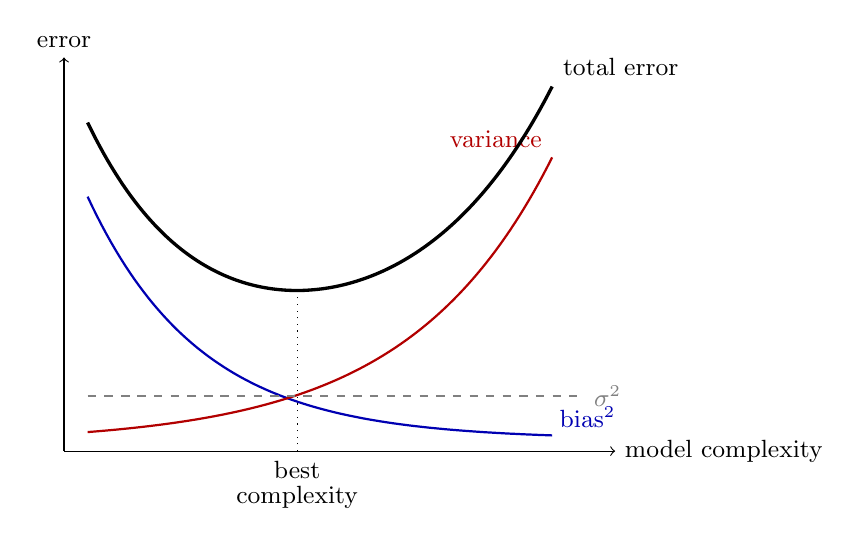
\begin{tikzpicture}[scale=1.0]
    % axes
    \draw[->] (0,0) -- (7,0) node[right] {\small model complexity};
    \draw[->] (0,0) -- (0,5) node[above] {\small error};
    % bias^2 : decreasing
    \draw[thick, blue!70!black, domain=0.3:6.2, samples=100]
        plot (\x, {3.8*exp(-0.7*\x)+0.15}) node[above right=-1pt, blue!70!black] {\small bias$^2$};
    % variance : increasing
    \draw[thick, red!70!black, domain=0.3:6.2, samples=100]
        plot (\x, {0.12*exp(0.55*\x)+0.1}) node[above left] {\small variance};
    % irreducible noise : constant
    \draw[thick, gray, dashed, domain=0.3:6.6]
        plot (\x, {0.7}) node[right, gray] {\small $\sigma^2$};
    % total error : U-shape (sum)
    \draw[very thick, black, domain=0.3:6.2, samples=120]
        plot (\x, {3.8*exp(-0.7*\x)+0.15 + 0.12*exp(0.55*\x)+0.1 + 0.7})
        node[above right] {\small total error};
    % sweet spot (minimum of the total curve, at x = ln(2.66/0.066)/1.25)
    \draw[dotted] (2.96,0) -- (2.96,2.04);
    \node[below] at (2.96,0) {\small \shortstack{best\\complexity}};
\end{tikzpicture}
\end{center}

\paragraph{Link with regularisation.}
This is exactly the knob that ridge regression turns. Increasing the regularisation
strength $\lambda$ shrinks the weights, which makes the predictor less sensitive to
the data (\emph{lower variance}) at the cost of pulling it away from any single
dataset's fit (\emph{higher bias}). Tuning $\lambda$ is therefore a direct way to
navigate the bias-variance tradeoff, and the optimal $\lambda$ is the one balancing
the two.

\begin{remark}[Why ``more of a theorem'']
Nothing in the derivation used the squared loss being applied to a \emph{linear}
model, nor even that $\hat f$ comes from least squares: the decomposition holds for
\emph{any} learning procedure $\mathcal{D} \mapsto \hat f$, as long as the error is
measured in squared loss. This is what makes the bias-variance tradeoff a general
lens rather than a fact about one algorithm.
\end{remark}


\subsection{Working it out for least squares and ridge}
\label{subsec:bv-ridge}

Everything so far has been abstract: bias and variance were defined but never
computed. For the two procedures of \Cref{subsec:ridge} they can be computed exactly,
in a few lines, and the answer is worth the effort: it turns the qualitative U-curve
into a formula, and it delivers one genuinely surprising conclusion.

\paragraph{The setting.}
We simplify in two ways, both standard. First, the design is \emph{fixed}: the inputs
$x_1, \dots, x_n$ are deterministic and only the noise is random, so
\[
y = X w^\star + \varepsilon , \qquad \E[\varepsilon] = 0, \qquad
\E[\varepsilon \varepsilon^\top] = \sigma^2 I_n .
\]
Second, the model is \emph{well specified}: the truth really is linear,
$f^\star(x) = \langle w^\star, x \rangle$ for some $w^\star \in \R^d$. Note the shift
of meaning, which is the usual convention in statistics but worth flagging: in this
subsection $w^\star$ is the \emph{true} parameter, matching the star of $f^\star$,
whereas in \Cref{subsec:ridge} it denoted a minimiser of the empirical risk. Fitted
quantities carry a hat here, as in $\hat w$. We measure the
error \emph{in sample}, that is, averaged over the training inputs themselves:
\[
\mathcal{E}(\hat w) \ \coloneqq \ \frac{1}{n} \sum_{i=1}^n
\E\Big[ \big( \langle \hat w, x_i \rangle - f^\star(x_i) \big)^2 \Big]
\ = \ \frac{1}{n}\, \E \big\Vert X \hat w - X w^\star \big\Vert^2 .
\]
This is the quantity of the theorem above, averaged over $x_0 \in \{x_1, \dots, x_n\}$
and with the constant $\sigma^2$ removed; it splits into bias$^2$ plus variance in
exactly the same way.

\paragraph{Ordinary least squares: no bias, and a variance you can read off.}

\begin{prop}[In-sample error of least squares]
\label{prop:bv-ols}
Assume $\rank(X) = d$, so that $\hat w = (X^\top X)^{-1} X^\top y$ is well defined.
Then $\hat w$ is \emph{unbiased}, $\E[\hat w] = w^\star$, so the bias vanishes at every
point, and
\[
\boxed{\ \mathcal{E}(\hat w) = \underbrace{0}_{\mathrm{bias}^2} \ + \
\underbrace{\frac{\sigma^2 d}{n}}_{\mathrm{variance}} \ } .
\]
\end{prop}

\begin{proof}
Substituting $y = X w^\star + \varepsilon$ into the closed form,
\[
\hat w = (X^\top X)^{-1} X^\top (X w^\star + \varepsilon)
= w^\star + (X^\top X)^{-1} X^\top \varepsilon ,
\]
and taking expectations gives $\E[\hat w] = w^\star$ since $\E[\varepsilon] = 0$.
Hence $X\hat w - X w^\star = \Pi \varepsilon$, where $\Pi \coloneqq X (X^\top X)^{-1}
X^\top$ is the orthogonal projector onto the column space of $X$ (this is the
projection met in the geometric interpretation of least squares). Therefore
\[
\mathcal{E}(\hat w) = \frac1n \E \Vert \Pi \varepsilon \Vert^2
= \frac1n \E\big[ \varepsilon^\top \Pi \varepsilon \big]
= \frac{\sigma^2}{n} \tr(\Pi) = \frac{\sigma^2 d}{n} ,
\]
using $\Pi^\top \Pi = \Pi$ and $\tr(\Pi) = \rank(X) = d$ for a projector.
\end{proof}

This one formula contains most of the intuition of the whole chapter. The error is
$\sigma^2 d / n$: it grows \emph{linearly with the number of features} and decays like
$1/n$. Each extra feature buys one more direction in which the estimator can chase the
noise, at a cost of exactly $\sigma^2/n$, and it is worth paying only if that feature
removes at least as much bias. This is the bias-variance tradeoff, made arithmetic.
Notice also what happens as $d$ approaches $n$: the error tends to $\sigma^2$, as large
as the noise itself, which is the first hint of the spike we will meet in
\Cref{subsec:double-descent}.

\paragraph{Ridge: paying bias to buy variance.}
For ridge nothing is unbiased any more, and the clean way to see both terms at once is
to diagonalise. Let
\[
X^\top X = \sum_{j=1}^d \mu_j\, u_j u_j^\top
\]
be an eigendecomposition, with eigenvalues $\mu_1, \dots, \mu_d \geq 0$ and
orthonormal eigenvectors $u_1, \dots, u_d$, and write $c_j \coloneqq \langle u_j,
w^\star \rangle$ for the coordinates of the truth in that basis. (In this subsection we
call the eigenvalues $\mu_j$, and not $\lambda_j$ as one normally would, because
$\lambda$ is already the regularisation strength. In \Cref{subsec:pca}, where no
regularisation appears, they go back to being $\lambda_j$.)

\begin{prop}[In-sample error of ridge]
\label{prop:bv-ridge}
For $\hat w_\lambda = (X^\top X + n\lambda I)^{-1} X^\top y$ and any $\lambda > 0$,
\[
\mathcal{E}(\hat w_\lambda)
= \underbrace{n \lambda^2 \sum_{j=1}^d \frac{\mu_j\, c_j^2}{(\mu_j + n\lambda)^2}}_{\mathrm{bias}^2(\lambda)}
\ + \ \underbrace{\frac{\sigma^2}{n} \sum_{j=1}^d \frac{\mu_j^2}{(\mu_j + n\lambda)^2}}_{\mathrm{variance}(\lambda)} .
\]
The first sum increases from $0$ to $\tfrac1n \Vert X w^\star\Vert^2$ as $\lambda$ goes
from $0$ to $\infty$; the second decreases from $\sigma^2 d / n$ to $0$.
\end{prop}

\begin{proof}
Write $M_\lambda \coloneqq (X^\top X + n \lambda I)^{-1}$, so that $\hat w_\lambda =
M_\lambda X^\top y = M_\lambda X^\top X w^\star + M_\lambda X^\top \varepsilon$. Taking
expectations and using $M_\lambda X^\top X = I - n\lambda M_\lambda$,
\[
\E[\hat w_\lambda] - w^\star = - n \lambda\, M_\lambda w^\star ,
\qquad
\hat w_\lambda - \E[\hat w_\lambda] = M_\lambda X^\top \varepsilon .
\]
The first identity gives the bias term: since $M_\lambda w^\star = \sum_j c_j (\mu_j +
n\lambda)^{-1} u_j$,
\[
\mathrm{bias}^2 = \frac1n \big\Vert X \cdot n\lambda M_\lambda w^\star \big\Vert^2
= n \lambda^2 \, (M_\lambda w^\star)^\top X^\top X\, (M_\lambda w^\star)
= n\lambda^2 \sum_{j=1}^d \frac{\mu_j c_j^2}{(\mu_j + n\lambda)^2} .
\]
The second gives the variance term:
\[
\mathrm{variance} = \frac1n \E \big\Vert X M_\lambda X^\top \varepsilon \big\Vert^2
= \frac{\sigma^2}{n} \tr\big( M_\lambda X^\top X M_\lambda X^\top X \big)
= \frac{\sigma^2}{n} \sum_{j=1}^d \frac{\mu_j^2}{(\mu_j + n\lambda)^2} .
\]
Both monotonicity statements are read off term by term, and the stated limits follow
from $\sum_j \mu_j c_j^2 = \Vert X w^\star \Vert^2$ and, when $\rank(X) = d$, from
$\mu_j > 0$ for every $j$.
\end{proof}

The two sums are the two arms of the U-curve, now completely explicit, and one sees
precisely how $\lambda$ trades them off: every eigendirection $j$ is shrunk by the
factor $\mu_j / (\mu_j + n\lambda) \in (0,1)$, which is close to $1$ for the directions
the data determines well ($\mu_j \gg n\lambda$, barely touched) and close to $0$ for
those it determines badly ($\mu_j \ll n\lambda$, essentially switched off). Ridge does
not shrink uniformly: it discards exactly the directions in which the data is
uninformative, which is precisely what the minimum-norm rule was doing implicitly in
\Cref{subsec:overparam}.

\paragraph{The surprise: $\lambda = 0$ is never optimal.}

\begin{corollary}[A little regularisation always helps]
\label{cor:ridge-beats-ols}
Assume $\rank(X) = d$ and $\sigma^2 > 0$. Then, as a function of $\lambda$, the
in-sample error satisfies
\[
\frac{\mathrm{d}}{\mathrm{d}\lambda} \, \mathcal{E}(\hat w_\lambda) \Big|_{\lambda = 0}
= - 2 \sigma^2 \sum_{j=1}^d \frac{1}{\mu_j} \ < \ 0 .
\]
In particular there exists $\lambda > 0$ with $\mathcal{E}(\hat w_\lambda) <
\mathcal{E}(\hat w_0) = \sigma^2 d / n$: \emph{some} amount of ridge regularisation
strictly beats ordinary least squares, whatever the data and whatever the truth
$w^\star$.
\end{corollary}

\begin{proof}
Set $u = n\lambda$. Near $u = 0$ the bias term is $\tfrac{u^2}{n}\sum_j \mu_j c_j^2
\mu_j^{-2} + O(u^3)$, so it is $O(u^2)$ and its derivative at $u = 0$ vanishes: the
bias costs nothing \emph{to first order}. The variance term, on the other hand, has
derivative $\tfrac{\sigma^2}{n} \sum_j (-2)\mu_j^2 (\mu_j + u)^{-3}$, equal to
$-\tfrac{2\sigma^2}{n}\sum_j \mu_j^{-1}$ at $u = 0$: it decreases at a strictly
positive rate. Multiplying by $\mathrm{d}u/\mathrm{d}\lambda = n$ gives the claim.
\end{proof}

This is worth pausing on, because it is not what one expects. Least squares is
unbiased, and unbiasedness sounds like a virtue; the corollary says it is the wrong
thing to optimise. Starting from $\lambda = 0$, a small penalty buys a first-order
reduction in variance for only a second-order increase in bias, so the trade is always
favourable at the start. The size of the gain is governed by $\sum_j 1/\mu_j$, which is
enormous exactly when $X^\top X$ has small eigenvalues, i.e.\ when the features are
nearly collinear and the least-squares fit is unstable. That is the regime where
practitioners reach for ridge, and this is the calculation that justifies them.

\begin{remark}[What the calculation does \emph{not} say]
Note that \Cref{cor:ridge-beats-ols} guarantees the existence of a good $\lambda$; it
does not tell us its value, which depends on the unknowns $\sigma^2$ and $w^\star$.
Choosing $\lambda$ in practice is done by cross-validation (\Cref{subsec:cv}), not by
this formula. What the formula gives is the reassurance that the search is not in vain,
and an understanding of when it will pay off most.
\end{remark}


\subsection{A puzzle: what about over-parametrised models?}
\label{subsec:double-descent}

At this point you should be suspicious. In \Cref{subsec:overparam} we insisted that
the regime $d > n$ is ``the rule rather than the exception in modern machine
learning'': the networks that work best in practice have far more parameters than
training samples, and they interpolate their training data exactly. But the U-curve
we have just drawn says that such models sit at the far right of the complexity axis,
drowning in variance, and should therefore be catastrophic. They are not. What is
going on?

The resolution is that \emph{``complexity'' was never the same thing as ``number of
parameters''}. The horizontal axis of the U-curve measures how much a procedure
can wobble when the data changes, and the derivation above bounds nothing about how
that relates to $d$. What the bias-variance theorem decomposes is the error of a
\emph{learning procedure}, dataset $\mapsto$ predictor, and adding parameters changes
that procedure in two ways at once:
\begin{itemize}
    \item it enlarges the function class $\F$, which is the effect the U-curve has in
    mind, and which does push the variance up;
    \item but once $d > n$ it also makes the minimiser \emph{non-unique}, and the
    procedure is then defined only by the extra rule we use to choose among the
    interpolants. In our case that rule is the minimum-norm one, reached either
    explicitly (ridge, as $\lambda \to 0^+$) or implicitly (gradient descent from
    $w_0 = 0$).
\end{itemize}
That second effect works in the \emph{opposite} direction. The more features we add
beyond $n$, the larger the space $\ker(X)$ of directions the data says nothing about,
and the harder the minimum-norm rule is pushing back towards $0$ along all of them.
Adding parameters past the interpolation threshold therefore keeps enriching the
class while \emph{also} strengthening the implicit regularisation, and the variance
can start going down again.

The empirical shape that results is called \emph{double descent}: as $d$ grows the
test error first traces the classical U-curve, then \emph{spikes} around the
interpolation threshold $d \approx n$ (where $X$ is barely invertible, $\Vert
w^\dagger \Vert$ blows up, and the fit is maximally unstable), and then descends a
\emph{second} time in the over-parametrised regime $d \gg n$, sometimes going below
the best error of the first descent.

\begin{remark}[The moral]
The bias-variance decomposition is a theorem and remains exactly true in the
over-parametrised regime: the test error is still noise plus bias$^2$ plus variance.
What is \emph{not} a theorem, and what modern practice violates, is the folklore that
variance increases monotonically with the number of parameters. This is why the
implicit bias of gradient descent, proved in \Cref{subsec:gd}, is not a curiosity: in
the over-parametrised regime it \emph{is} the regularisation, and it is what decides
whether a model that interpolates its training data generalises or not.
\end{remark}


\subsection{Estimating the test error: validation and cross-validation}
\label{subsec:cv}

Everything above is about a quantity, the test error, that we have never explained
how to \emph{compute}. This is not a detail: the whole discussion tells us to pick the
model complexity, or the ridge parameter $\lambda$, at the bottom of the U-curve, and
we cannot do that without a number to minimise. The decomposition itself is of no help
here, since $f^\star$ and $\sigma^2$ are unknown. What follows is how it is done in
practice, and it is the single most used recipe in all of machine learning.

\paragraph{Why the training error will not do.}
The obvious candidate, the empirical risk $L(\hat w)$ on the data we fitted on, is
useless, and the two extremes above show exactly why: it can be driven to zero by a
procedure that generalises terribly. The reason is that $\hat w$ was \emph{chosen
using} those very points, so the residuals on them are not representative. Any
estimate of the test error must be computed on data the fitting procedure has
not seen.

\paragraph{The train / validation / test split.}
The remedy is to spend our $n$ samples on three different jobs, splitting them at
random into three disjoint parts.
\begin{itemize}
    \item The \emph{training set} (say $60\%$) is used to fit $\hat w$, for each
    candidate value of the quantity we are trying to choose (the polynomial degree
    $k$, the ridge parameter $\lambda$, \dots). Such a quantity, which is not fitted by
    the optimiser but selected from outside, is called a \emph{hyperparameter}.
    \item The \emph{validation set} (say $20\%$) is used to \emph{compare} those
    fitted models: we evaluate the squared error of each on it and keep the
    hyperparameter achieving the smallest one. This is our estimate of the U-curve,
    and its minimiser is our estimate of the best complexity.
    \item The \emph{test set} (say $20\%$) is locked away until the very end and used
    exactly once, to report the error of the final model.
\end{itemize}

\begin{remark}[Why a third set is needed]
The last point is the one most often skipped, and it matters. Once we have minimised
the validation error over, say, twenty values of $\lambda$, the winning value was
selected \emph{because} it did well on the validation set, and part of why it did well
is luck specific to those points. The validation error of the winner is therefore
optimistically biased, for exactly the same reason the training error was: it is the
minimum over many noisy quantities. The test set is untouched by any choice we made,
so it gives an honest number. A useful way to put it: the validation set is used to
\emph{choose}, the test set only to \emph{report}.
\end{remark}

\paragraph{$K$-fold cross-validation.}
A single validation set is wasteful when $n$ is small: we throw away $20\%$ of the
data when fitting, and the resulting estimate is itself noisy, since it depends on
which points happened to land in the validation part. \emph{Cross-validation} fixes
both problems by rotating the role of the validation set. Split the training data into
$K$ disjoint blocks (\emph{folds}) $I_1, \dots, I_K$ of roughly equal size. Then, for
each fold $k = 1, \dots, K$:
\begin{itemize}
    \item fit the model on everything \emph{except} $I_k$, giving a parameter
    $\hat w^{(-k)}$;
    \item evaluate the error on the held-out fold $I_k$, which was not used for that
    fit,
    \[
    e_k = \frac{1}{|I_k|} \sum_{i \in I_k}
    \big( \langle \hat w^{(-k)}, x_i \rangle - y_i \big)^2 .
    \]
\end{itemize}
The cross-validation score is the average $\mathrm{CV} = \tfrac{1}{K} \sum_{k=1}^K
e_k$, and we choose the hyperparameter minimising it. Every point is used for fitting
in $K-1$ of the folds and for evaluation in exactly one, so no data is wasted and the
averaging over $K$ folds reduces the variance of the estimate. The price is that we
now fit $K$ models per hyperparameter value instead of one.

Typical choices are $K = 5$ or $K = 10$. The extreme case $K = n$, in which each fold
is a single point, is called \emph{leave-one-out} cross-validation: it uses the data
maximally but requires $n$ fits, which is usually prohibitive.

\begin{remark}[Two traps]
\emph{Split before you preprocess.} Any quantity estimated from the data, in
particular the feature means and standard deviations used for standardisation, must be
computed on the training part only and then applied to the validation and test parts.
Standardising the full dataset first lets information about the held-out points leak
into the fit, and the resulting estimate is again optimistic; see
\Cref{subsec:standardise}. \emph{Split
respecting the structure of the data.} The reasoning above assumes the samples are
independent. For time series, or when several samples come from the same patient or
the same user, a uniformly random split puts near-duplicates on both sides and makes
the estimate meaningless; one splits by time, or by patient, instead.
\end{remark}

\begin{exercise}[$\star$]
Take the polynomial model of degree $k$ on a small dataset. Plot, as functions of $k$,
the training error and the $5$-fold cross-validation error on the same axes. Which one
is U-shaped? Which one is monotone, and in which direction? Compare with the figure
above.
\end{exercise}


\newpage
\section{Unsupervised learning}
\label{sec:unsupervised}

Everything so far has been supervised: every input $x_i$ came with a label $y_i$, and
the whole machinery was built to predict $y$ from $x$. We now remove the labels.

\subsection{The setup, and what changes without labels}
\label{subsec:unsup-setup}

The data is a plain collection of points
\[
x_1, \dots, x_n \in \R^d ,
\]
with nothing attached to them, and we stack them as always into the design matrix
$X \in \R^{n \times d}$ whose $i$-th row is $x_i$. There is no $y$, and therefore
no function $f$ to fit and no prediction to be scored. The question becomes the vaguer
one of \emph{finding structure}: is the cloud of points really spread over all $d$
directions, or does it essentially live in a much smaller subspace? Does it break up
into a few well-separated groups?

\paragraph{What we keep: one recipe, two instances.}
The good news is that the main ideas of these notes stay mostly intact. We still
write down a class of simplified descriptions of the data, still measure quality by a
squared error, and still minimise. The unifying statement, which is the thread running
through this whole section, is that both methods we study solve
\[
\ \min_{\hat X \,\in\, \mathcal{C}} \ \big\Vert X - \hat X \big\Vert_F^2 
\]
for two different choices of the set $\mathcal{C}$ of allowed reconstructions
$\hat X \in \R^{n \times d}$. In both cases $\hat X$ is a \emph{simplified stand-in}
for the data: row $i$ of $\hat X$ is what we keep of the point $x_i$, and the objective
asks that we lose as little as possible.
\begin{itemize}
    \item \emph{Principal component analysis} takes $\mathcal{C}$ to be the matrices
    whose rows all lie in one $K$-dimensional linear subspace of $\R^d$. Each point is
    replaced by its projection onto a common subspace: the data is compressed in
    \emph{direction}.
    \item \emph{$K$-means} takes $\mathcal{C}$ to be the matrices whose rows take at
    most $K$ distinct values. Each point is replaced by the centroid of its group: the
    data is compressed in \emph{identity}, since after the reconstruction all we
    remember of $x_i$ is which of $K$ representatives it was closest to.
\end{itemize}
The parameter $K$ measures, in both cases, how much we allow ourselves to keep, and it
is a hyperparameter we must pick: it is not fitted by the
optimiser.

\begin{remark}[The Frobenius norm]
\label{rem:frobenius}
The norm above is the \emph{Frobenius} norm, which is nothing more exotic than the
Euclidean norm of a matrix read as a long vector:
\[
\Vert A \Vert_F^2 \ \coloneqq \ \sum_{i,j} A_{i,j}^2 \ = \ \tr(A^\top A) .
\]
When the rows of $A$ are $a_1, \dots, a_n$ this is $\sum_{i=1}^n \Vert a_i \Vert^2$, so
$\Vert X - \hat X \Vert_F^2 = \sum_{i=1}^n \Vert x_i - \hat x_i \Vert^2$ really is the
total squared reconstruction error, summed over the samples. We use throughout the
\emph{cyclicity of the trace}, $\tr(AB) = \tr(BA)$ whenever both products are defined;
see \Cref{sec:cheat-linalg}.
\end{remark}

\begin{remark}[A third index]
\label{rem:third-index}
Both methods need to count \emph{groups} (clusters, or directions kept), a third kind
of index alongside the samples $i$ and the coordinates $j$ used throughout these notes. We
use $k$ for it, ranging over $1, \dots, K$, exactly as $k$ already ranged over the
classes in \Cref{sec:classification}. So $x_i$ is a sample, $x_{i,j}$ one of its
coordinates, and $\mu_k$ or $v_k$ the $k$-th centroid or direction.
\end{remark}


\subsection{Principal component analysis}
\label{subsec:pca}

\paragraph{Centring.}
PCA is about \emph{directions of variation}, so the position of the cloud is
irrelevant and must be removed first. Throughout this subsection we assume the data has
been \emph{centred}: writing $\bar x = \tfrac1n \sum_{i=1}^n x_i$ for the empirical
mean, we replace each $x_i$ by $x_i - \bar x$, so that
\[
\frac{1}{n} \sum_{i=1}^n x_i = 0 ,
\]
and we keep calling the resulting matrix $X$. This is an important step: without it
the first principal direction is dominated by the direction of $\bar x$, which says
where the data sits rather than how it varies. Whether one should further
\emph{standardise} the coordinates is a separate and more debatable question, discussed
at the end of the subsection.

\paragraph{Projecting onto a subspace.}
We look for a linear subspace $S \subseteq \R^d$ of dimension $K \leq d$ on which to
project the data. Describe it by an orthonormal basis $v_1, \dots, v_K$, that is,
$\langle v_k, v_{k'} \rangle = \delta_{k,k'}$, and gather the basis into a matrix
\[
V = \big( v_1 \mid \dots \mid v_K \big) \in \R^{d \times K} ,
\qquad \text{so that} \qquad
V^\top V = I_K ,
\]
the last identity being exactly the statement that the columns are orthonormal.
Two matrices are then worth reading carefully, because everything follows from them.

The matrix $XV \in \R^{n \times K}$ collects the \emph{coordinates of the data in the
new basis}:
\[
XV = \begin{pmatrix}
\langle x_1, v_1 \rangle & \dots & \langle x_1, v_K \rangle \\
\vdots & & \vdots \\
\langle x_n, v_1 \rangle & \dots & \langle x_n, v_K \rangle
\end{pmatrix} .
\]
Its $i$-th row is the compressed version of $x_i$: $K$ numbers instead of $d$. These
are the \emph{scores}, or \emph{principal components}, of the data.

The matrix $X V V^\top \in \R^{n \times d}$ puts them back into the original space:
\[
X V V^\top = \begin{pmatrix}
- & \sum_{k=1}^K \langle x_1, v_k \rangle\, v_k & - \\
  & \vdots & \\
- & \sum_{k=1}^K \langle x_n, v_k \rangle\, v_k & -
\end{pmatrix} ,
\]
whose $i$-th row is the orthogonal projection of $x_i$ onto $S$. So $P_V \coloneqq
V V^\top \in \R^{d \times d}$ is the orthogonal projector onto $S$, and $\hat X = X
V V^\top$ is precisely the reconstruction of \Cref{subsec:unsup-setup}, with
$\mathcal{C}$ the set of matrices whose rows lie in a common $K$-dimensional subspace.

\begin{exercise}[$\star$]
Check that $P_V = VV^\top$ satisfies $P_V^\top = P_V$ and $P_V^2 = P_V$, so it is
indeed an orthogonal projector, and that $\rank(P_V) = K$. Where is $V^\top V = I_K$
used? Note that $V V^\top \neq I_d$ unless $K = d$: the order of the product matters
enormously.
\end{exercise}

\paragraph{The objective, and its two readings.}
PCA chooses the subspace minimising the reconstruction error:
\[
\min_{V \in \R^{d \times K}, \ V^\top V = I_K} \ \big\Vert X - X V V^\top \big\Vert_F^2 .
\]
The following computation, which is the heart of the matter, turns this into an
eigenvalue problem.

\begin{prop}[Reconstruction error and retained variance]
\label{prop:pca-two-readings}
For every $V \in \R^{d \times K}$ with $V^\top V = I_K$,
\[
\big\Vert X - X V V^\top \big\Vert_F^2
\ = \ \Vert X \Vert_F^2 \ - \ \tr\big( V^\top X^\top X\, V \big) .
\]
Since $\Vert X \Vert_F^2$ does not depend on $V$, \emph{minimising the reconstruction
error is the same problem as maximising} $\tr(V^\top X^\top X V)$.
\end{prop}

\begin{proof}
Expand the square using $\Vert A \Vert_F^2 = \tr(A^\top A)$:
\[
\big\Vert X - X V V^\top \big\Vert_F^2
= \tr(X^\top X) - 2\, \tr\big( X^\top X V V^\top \big)
+ \tr\big( V V^\top X^\top X V V^\top \big) ,
\]
where the cross terms were merged using $\tr(A^\top) = \tr(A)$. For the last term,
cyclicity of the trace moves the leading $V$ to the end,
\[
\tr\big( V V^\top X^\top X V V^\top \big) = \tr\big( V^\top X^\top X V \, V^\top V \big)
= \tr\big( V^\top X^\top X V \big) ,
\]
using $V^\top V = I_K$; and the same cyclicity gives $\tr(X^\top X V V^\top) =
\tr(V^\top X^\top X V)$. The two therefore combine into $-2 + 1 = -1$ times
$\tr(V^\top X^\top X V)$, which is the claim.
\end{proof}

The quantity being maximised has a direct statistical meaning. Since the data is
centred,
\[
\tr\big( V^\top X^\top X V \big) = \sum_{k=1}^K v_k^\top X^\top X\, v_k
= \sum_{k=1}^K \sum_{i=1}^n \langle x_i, v_k \rangle^2
= \big\Vert X V \big\Vert_F^2 ,
\]
which is $n$ times the total \emph{empirical variance of the projected data}. So the
two natural things one might have asked for turn out to be the same request:

\begin{center}
\begin{tabular}{@{}c@{\quad}c@{\quad}c@{}}
\emph{keep the subspace} & $\Longleftrightarrow$ & \emph{keep the subspace} \\
\emph{losing the least information} & & \emph{carrying the most variance.}
\end{tabular}
\end{center}

\noindent
This is the first thing to remember about PCA. It is also why the empirical covariance
matrix
\[
\hat \Sigma \ \coloneqq \ \frac{1}{n} X^\top X \ \in \R^{d \times d}
\]
is the object that decides everything: it is symmetric positive semi-definite (see
\Cref{sec:cheat-convexity}), and the problem is now to maximise $\tr(V^\top \hat\Sigma
V)$ over orthonormal $V$.

\paragraph{Solving it.}
Start with a single direction, where the answer is the classical Rayleigh quotient
bound.

\begin{lemma}[One direction]
\label{lem:rayleigh}
Let $A \in \R^{d \times d}$ be symmetric with eigenvalues $\lambda_1 \geq \dots \geq
\lambda_d$ and corresponding orthonormal eigenvectors $u_1, \dots, u_d$. Then
\[
\max_{\Vert v \Vert = 1} \ v^\top A v = \lambda_1 ,
\]
attained at $v = u_1$.
\end{lemma}

\begin{proof}
Write $v = \sum_{j=1}^d c_j u_j$ in the eigenbasis, so that $\Vert v \Vert^2 = \sum_j
c_j^2 = 1$. Then $v^\top A v = \sum_j \lambda_j c_j^2 \leq \lambda_1 \sum_j c_j^2 =
\lambda_1$, a weighted average of the eigenvalues being at most the largest. Equality
requires all the weight to sit on eigenvalues equal to $\lambda_1$, and $v = u_1$ works.
\end{proof}

The general case is the same statement one dimension at a time, and the proof is
pleasantly short once one thinks in terms of the projector rather than the basis.

\begin{thm}[PCA]
\label{thm:pca}
With $A = X^\top X$ symmetric positive semi-definite, with eigenvalues $\lambda_1 \geq
\dots \geq \lambda_d \geq 0$ and orthonormal eigenvectors $u_1, \dots, u_d$,
\[
\max_{V^\top V = I_K} \ \tr\big( V^\top X^\top X V \big) = \lambda_1 + \dots + \lambda_K ,
\]
attained by $V = (u_1 \mid \dots \mid u_K)$. The optimal subspace is therefore the span
of the $K$ leading eigenvectors of $X^\top X$, equivalently of the empirical covariance
$\hat\Sigma$, and the minimal reconstruction error is $\lambda_{K+1} + \dots +
\lambda_d$. The vectors $u_1, u_2, \dots$ are called the \emph{principal directions},
and $u_k$ the $k$-th one.
\end{thm}

\begin{proof}
Put $B = V V^\top$, the orthogonal projector onto the chosen subspace, and set
$\alpha_j \coloneqq u_j^\top B\, u_j$ for each $j$. Two observations:
\[
\alpha_j = \Vert V^\top u_j \Vert^2 \geq 0 ,
\qquad
\alpha_j \leq \Vert u_j \Vert^2 = 1 ,
\]
the second because an orthogonal projection never lengthens a vector, and
\[
\sum_{j=1}^d \alpha_j = \tr(B) = \tr(V V^\top) = \tr(V^\top V) = \tr(I_K) = K .
\]
Now expand $A = \sum_j \lambda_j u_j u_j^\top$ and use cyclicity again:
\[
\tr\big( V^\top A V \big) = \tr(A B) = \sum_{j=1}^d \lambda_j\, u_j^\top B u_j
= \sum_{j=1}^d \lambda_j \alpha_j .
\]
So the problem is bounded by the largest value of $\sum_j \lambda_j \alpha_j$ over all
$\alpha \in [0,1]^d$ with $\sum_j \alpha_j = K$. Since the $\lambda_j$ are sorted, the
best possible allocation of a total budget $K$ into weights capped at $1$ is to give a
full unit to each of the $K$ largest, giving $\lambda_1 + \dots + \lambda_K$. Taking
$V = (u_1 \mid \dots \mid u_K)$ gives exactly $\alpha_j = \mathbf{1}\{ j \leq K\}$, so
the bound is attained. Finally the minimal reconstruction error follows from
\Cref{prop:pca-two-readings} and $\Vert X \Vert_F^2 = \tr(X^\top X) = \sum_j \lambda_j$.
\end{proof}

\begin{remark}[The solution is nested, and the subspace is what matters]
The proof shows something the statement hides: the optimal $K$-dimensional subspace
\emph{contains} the optimal $(K-1)$-dimensional one. One does not re-solve the problem
for each $K$; one computes the eigenvectors once, sorted, and takes as many as one
wants. Note also that $V$ itself is not unique (any rotation of an orthonormal basis of
the same subspace gives the same reconstruction, and eigenvectors are only defined up
to sign), but the \emph{subspace} is, as soon as $\lambda_K > \lambda_{K+1}$.
\end{remark}

\begin{remark}[In practice one uses the SVD]
Forming $X^\top X$ and diagonalising it is the textbook route but not the numerical one,
for the reason given in \Cref{subsec:numerics}: it squares the condition number. Every
library instead computes the singular value decomposition $X = U D W^\top$, with $U \in
\R^{n \times n}$ and $W \in \R^{d \times d}$ orthogonal and $D \in \R^{n \times d}$ zero
off its diagonal, with diagonal entries $s_1 \geq s_2 \geq \dots \geq 0$. Then $X^\top X = W D^\top D W^\top$, so the principal
directions are the columns of $W$ (the right singular vectors) and $\lambda_k = s_k^2$.
The scores are $XV = U D$ restricted to the first $K$ columns.
\end{remark}

\paragraph{Choosing $K$.}
The eigenvalues answer this too, at least descriptively. The quantity
\[
\frac{\lambda_1 + \dots + \lambda_K}{\lambda_1 + \dots + \lambda_d} \ \in [0, 1]
\]
is the \emph{fraction of variance explained} by the first $K$ directions, and plotting
either it or the individual $\lambda_k$ against $k$ (a \emph{scree plot}) is the usual
way to decide. One looks for an elbow, a $K$ after which the eigenvalues fall off a
cliff, or simply takes the smallest $K$ explaining, say, $95\%$ of the variance. Both
are rules of thumb rather than theorems: there is no test error here to minimise. When
PCA is used as a preprocessing step before a supervised model, however, $K$ becomes an
ordinary hyperparameter of that model and can be chosen honestly by cross-validation.

\begin{remark}[Two warnings]
\emph{Centring is not optional, scaling is a modelling
choice.} PCA maximises variance, and variance has units: a feature measured in
millimetres has a variance $10^6$ times larger than the same feature in metres, and
will monopolise the first direction for no better reason. When the coordinates are
heterogeneous quantities one therefore standardises them first
(\Cref{subsec:standardise}), which amounts to diagonalising the empirical
\emph{correlation} matrix rather than the covariance. When all coordinates are
commensurate, as with the pixels of an image, standardising is usually the wrong thing
to do, since the differences in variance are then real information.
\end{remark}

\begin{exercise}[$\star$]
Take $d = 2$ and a cloud of points lying almost exactly on a line through the origin.
What are $\lambda_1, \lambda_2$ roughly, what is $u_1$, and what does the reconstruction
$X V V^\top$ look like for $K = 1$? Draw the picture.
\end{exercise}

\begin{exercise}[$\star\star$]
Show that PCA also solves the following apparently different problem: among all
matrices $\hat X$ of rank at most $K$, the one minimising $\Vert X - \hat X\Vert_F$ is
$\hat X = X V V^\top$ with $V$ as in \Cref{thm:pca}. (Start by checking that the rows of
$X V V^\top$ lie in a $K$-dimensional subspace, so $\rank(XVV^\top) \le K$; then argue
that any $\hat X$ of rank $\leq K$ has its rows in some $K$-dimensional subspace, and
that for a \emph{fixed} such subspace the best $\hat X$ is the orthogonal projection of
$X$ onto it.) This is a special case of the Eckart-Young theorem.
\end{exercise}


\subsection{$K$-means}
\label{subsec:kmeans}

We now compress in the other direction. Instead of asking that all the points be well
described by a common subspace, we ask that each point be well described by \emph{one
of $K$ representatives}.

\paragraph{The objective.}
Fix the hyperparameter $K$, the number of clusters. We look for
\begin{itemize}
    \item a \emph{partition} of the samples into $K$ groups $S_1, \dots, S_K$, i.e.\
    disjoint sets with $S_1 \cup \dots \cup S_K = \{1, \dots, n\}$;
    \item and $K$ \emph{centroids} $\mu_1, \dots, \mu_K \in \R^d$, one per group,
\end{itemize}
minimising the total squared distance from each point to the centroid of its own group,
\[
\mathcal{L}(S, \mu) \ = \ \sum_{k=1}^K \ \sum_{i \in S_k} \big\Vert x_i - \mu_k \big\Vert^2 .
\]
This is the natural way to say ``the groups should be tight''. Note that only the
squared Euclidean distance appears, which is already a modelling commitment: it is what
will make the clusters come out round.

\paragraph{Matrix form: the same problem as PCA, differently constrained.}
The partition is more conveniently encoded by an \emph{assignment matrix}. Let
\[
Z = (z_{i,k}) \in \{0, 1\}^{n \times K} , \qquad
\sum_{k=1}^K z_{i,k} = 1 \quad \text{for every } i ,
\]
so that $z_{i,k} = 1$ exactly when sample $i$ belongs to cluster $k$, each row of $Z$
containing a single $1$. Stack the centroids into
\[
M = \begin{pmatrix} - & \mu_1 & - \\ & \vdots & \\ - & \mu_K & - \end{pmatrix}
\in \R^{K \times d} .
\]
Then row $i$ of the product $ZM$ is $\sum_k z_{i,k} \mu_k$, which is simply the centroid
assigned to sample $i$, and therefore
\[
\mathcal{L}(M, Z)
= \sum_{i=1}^n \sum_{k=1}^K z_{i,k} \big\Vert x_i - \mu_k \big\Vert^2
= \big\Vert X - Z M \big\Vert_F^2 .
\]
So $K$-means is
\[
\min_{M \in \R^{K \times d}} \ \min_{\substack{Z \in \{0,1\}^{n \times K} \\ \sum_k z_{i,k} = 1 \ \forall i}}
\ \big\Vert X - Z M \big\Vert_F^2 ,
\]
which is exactly the reconstruction problem of \Cref{subsec:unsup-setup}: the
reconstruction is $\hat X = ZM$, whose rows take at most $K$ distinct values, namely the
$\mu_k$. Compare with PCA, where $\hat X = X V V^\top$ had rows in a $K$-dimensional
subspace. Same objective, same $K$, different notion of ``simple''.

\begin{exercise}[$\star$]
Check the middle equality above in detail: why does $\sum_k z_{i,k}\Vert x_i -
\mu_k\Vert^2$ equal $\Vert x_i - \sum_k z_{i,k}\mu_k\Vert^2$? (Use that exactly one term
of the sum is nonzero. Warning: this would be false for a general $Z$ with rows summing
to $1$ but entries in $[0,1]$ rather than $\{0,1\}$.)
\end{exercise}

\paragraph{The bad news.}
Unlike every problem we have met so far, this one is genuinely intractable: minimising
$\mathcal{L}$ jointly over $Z$ and $M$ is \textbf{NP-hard}, already for $d = 2$. The
reason is visible in the formulation: $Z$ ranges over a \emph{discrete} set, of size
$K^n$, and no amount of convexity is going to help, since the objective is not even
defined on a continuum. Exhaustive search is hopeless, and there is no closed form and
no gradient descent to fall back on.

\paragraph{The good news: alternating minimisation.}
What saves the situation is that although the joint problem is hard, each of the two
variables is easy \emph{given the other}, and in both cases the partial minimisation has
a closed form. That suggests the obvious algorithm: minimise alternately in $Z$ and in
$M$. This is \emph{Lloyd's algorithm}, universally called ``the'' $K$-means algorithm.

\begin{lemma}[The two steps]
\label{lem:kmeans-steps}
\emph{(Assignment.)} For a fixed $M$, the minimiser over admissible $Z$ is obtained
independently for each sample by assigning it to its nearest centroid:
\[
z_{i,k} = 1 \quad \text{if} \quad k = \argmin_{1 \leq k' \leq K} \ \big\Vert x_i - \mu_{k'} \big\Vert ,
\]
ties broken arbitrarily.

\emph{(Update.)} For a fixed $Z$, with associated groups $S_k = \{ i : z_{i,k} = 1\}$
assumed non-empty, the minimiser over $M$ is obtained independently for each cluster by
taking the mean of its points:
\[
\mu_k = \frac{1}{|S_k|} \sum_{i \in S_k} x_i
= \frac{\sum_{i=1}^n z_{i,k}\, x_i}{\sum_{i=1}^n z_{i,k}} .
\]
\end{lemma}

\begin{proof}
For the assignment step, write $\mathcal{L}(M, Z) = \sum_{i=1}^n \big( \sum_k z_{i,k}
\Vert x_i - \mu_k\Vert^2 \big)$. The constraint couples nothing across samples: each
row of $Z$ is chosen separately, and since that row must put its single $1$ somewhere,
the best place is the smallest of the $K$ numbers $\Vert x_i - \mu_k \Vert^2$.

For the update step, the objective splits as $\sum_{k=1}^K \big( \sum_{i \in S_k} \Vert
x_i - \mu_k \Vert^2 \big)$, and each bracket involves only $\mu_k$. So we must minimise
$\mu \mapsto \sum_{i \in S} \Vert x_i - \mu \Vert^2$ for a fixed set $S$. This is a
quadratic function of $\mu$, with Hessian $2 |S|\, I_d \succ 0$, hence strictly convex,
so its unique minimiser is the point where its gradient vanishes:
\[
\nabla_\mu \sum_{i \in S} \Vert x_i - \mu \Vert^2
= - 2 \sum_{i \in S} \big( x_i - \mu \big)
= 2 \Big( |S|\, \mu - \sum_{i \in S} x_i \Big) = 0
\quad \Longleftrightarrow \quad
\mu = \frac{1}{|S|} \sum_{i \in S} x_i ,
\]
which is the announced mean.
\end{proof}


\begin{center}
\fbox{\parbox{0.9\textwidth}{
\textbf{Lloyd's algorithm.} Initialise the centroids $\mu_1^{(0)}, \dots, \mu_K^{(0)}
\in \R^d$. Then for $t = 0, 1, 2, \dots$ repeat:
\begin{enumerate}
    \item \emph{Assignment.} $Z^{(t+1)} = \argmin_Z \ \mathcal{L}(M^{(t)}, Z)$: assign
    each sample to its nearest current centroid.
    \item \emph{Update.} $M^{(t+1)} = \argmin_M \ \mathcal{L}(M, Z^{(t+1)})$: replace
    each centroid by the mean of the samples just assigned to it.
\end{enumerate}
Stop when the assignment no longer changes.
}}
\end{center}

\paragraph{Why it stops.}
The convergence argument is unusual and pleasantly elementary: it is not an analytic
statement about small step sizes, but a counting argument.

\begin{prop}[Convergence in finitely many steps]
\label{prop:lloyd-converges}
The sequence $\mathcal{L}(M^{(t)}, Z^{(t)})$ is non-increasing and bounded below by $0$.
Moreover Lloyd's algorithm terminates after finitely many iterations.
\end{prop}

\begin{proof}
Each of the two steps minimises $\mathcal{L}$ in one variable with the other held fixed,
so neither can increase it:
\[
\mathcal{L}\big(M^{(t)}, Z^{(t)}\big) \ \geq \ \mathcal{L}\big(M^{(t)}, Z^{(t+1)}\big)
\ \geq \ \mathcal{L}\big(M^{(t+1)}, Z^{(t+1)}\big) ,
\]
and $\mathcal{L} \geq 0$ as a sum of squares. For termination, note that after the
update step the centroids are \emph{determined} by the assignment, so from $t \geq 1$
onwards the value $\mathcal{L}(M^{(t)}, Z^{(t)})$ is a function of $Z^{(t)}$ alone. There are at most
$K^n$ admissible assignment matrices, hence finitely many possible values. A
non-increasing sequence taking finitely many values is eventually constant; and as soon
as the value fails to decrease strictly, the assignment step has returned the same $Z$
and the algorithm has stopped by its own criterion.
\end{proof}

\begin{remark}[Stopping is not succeeding]
\Cref{prop:lloyd-converges} guarantees termination, and nothing more. The point reached
is a \emph{local} minimum, in the weak sense that neither step alone can improve it, and
it can be arbitrarily worse than the global one: it is easy to draw four obvious
clusters and an initialisation from which Lloyd's algorithm splits one of them in two
and merges another two, then stops, perfectly stable and perfectly wrong. This is
exactly the difficulty that convexity spared us throughout the supervised part of these
notes, and there is no way around it here.

The standard remedies are (i) to run the algorithm several times from different random
initialisations and keep the run with the smallest final $\mathcal{L}$, which is cheap
and is what libraries do by default, and (ii) to initialise cleverly rather than
uniformly at random, spreading the initial centroids out. The latter is the
\emph{$K$-means$++$} initialisation: pick the first centroid uniformly among the data
points, then each subsequent one at random with probability proportional to the squared
distance to the nearest centroid already chosen. It costs almost nothing and improves
results markedly.
\end{remark}

\paragraph{What can go wrong.}
Beyond the local minima, three limitations are worth knowing, all of them consequences
of the squared Euclidean distance in the objective.
\begin{itemize}
    \item \emph{The number of clusters must be given.} $K$ is a hyperparameter, and
    unlike in the supervised setting there is no held-out error to select it: the
    objective $\mathcal{L}$ decreases mechanically as $K$ grows, reaching $0$ at $K = n$,
    so it cannot be used to choose $K$ either. The usual device is again an
    \emph{elbow plot} of the final $\mathcal{L}$ against $K$, looking for the point
    where the curve flattens.
    \item \emph{The clusters come out round, and of comparable size.} Minimising squared
    distances to a centre means the implied shape is a ball, and the boundary between
    two clusters is the hyperplane bisecting the segment between their centroids. Two
    interleaved crescents, or one long thin cluster next to a round one, will be cut in
    a way no human would choose. If the natural groups are not blobs, $K$-means is the
    wrong tool.
    \item \emph{Outliers hurt twice.} A single far-away point contributes an enormous
    squared distance, so it drags the centroid of whichever cluster adopts it, and it may
    even claim a whole cluster for itself. Squared errors are not robust, exactly as in
    \Cref{sec:regression}.
\end{itemize}
To which one should add the familiar warning that the Euclidean distance mixes the
coordinates, so features on wildly different scales must be standardised first.

\begin{exercise}[$\star$]
Why does $\min \mathcal{L}$ decrease as $K$ increases? (Show that any solution with $K$
clusters can be turned into one with $K+1$ clusters and no larger loss.) Deduce that
choosing $K$ by minimising $\mathcal{L}$ would always return $K = n$.
\end{exercise}

\begin{exercise}[$\star\star$]
Take $n = 4$ points in $\R^2$ at the corners of a rectangle that is much wider than it
is tall, and $K = 2$. Find the global minimiser. Then exhibit an initialisation of the
centroids from which Lloyd's algorithm converges to the other, worse, partition.
\end{exercise}




% \newpage
% \section{The probabilistic view}
\label{sec:probabilistic}

Every method in these notes was introduced the same way: we chose a function class, we
chose a loss, and we minimised. The choice of loss was always motivated, but always
somewhat by hand. The squared error was ``by far the most common''; the logistic loss
won a beauty contest against three rivals; the $K$-means objective simply asserted that
groups should be tight. The reader is entitled to ask where these expressions actually
come from, and whether there is any principle behind them or only tradition.

There is a principle, and this section is about it. In every case, the objective we
minimised is the \emph{negative log-likelihood} of an explicit probabilistic model of
how the data was generated. Different losses are not competing conventions: they are
different assumptions about the data, written in a different alphabet. This is worth a
section of its own for three reasons. It explains where our losses come from; it tells
us how to build a new one when the standard assumptions do not fit; and it delivers
something the risk-minimisation view never gave us, namely predictions that come with
probabilities attached rather than bare numbers.

\subsection{Maximum likelihood in one page}
\label{subsec:mle}

\paragraph{The principle.}
Suppose we posit a family of probability distributions $p_\theta$, indexed by a
parameter $\theta$, as candidate explanations for how the data was produced. Having
observed data $\mathcal{D}$, the \emph{likelihood} of $\theta$ is the probability (or
density) that the model assigns to what we actually saw,
\[
\theta \ \longmapsto \ p_\theta(\mathcal{D}) .
\]
\emph{Maximum likelihood estimation} (MLE) picks the parameter making the observed data
as unsurprising as possible:
\[
\hat\theta \ \in \ \argmax_{\theta} \ p_\theta(\mathcal{D}) .
\]
Note the logic, which students often reverse: the data is fixed and the parameter
varies. The likelihood is \emph{not} a probability distribution over $\theta$.

\paragraph{Why the logarithm, and why the minus sign.}
If the $n$ samples are independent, the likelihood is a product, and products are
unpleasant: they underflow, and their derivatives are a mess. Since $\log$ is strictly
increasing, maximising $p_\theta(\mathcal{D})$ is the same as maximising $\log
p_\theta(\mathcal{D})$, which turns the product into a sum. Flipping the sign to get a
minimisation, as is our habit, gives the \emph{negative log-likelihood}
\[
\mathrm{NLL}(\theta) \ = \ - \log p_\theta(\mathcal{D})
\ = \ - \sum_{i=1}^n \log p_\theta(\text{sample } i) ,
\]
and dividing by $n$, which does not move the minimiser (the same remark as in
\Cref{sec:regression}), puts it in exactly the shape of an empirical risk:
\[
\boxed{\
\frac{1}{n}\, \mathrm{NLL}(\theta)
\ = \ \frac{1}{n} \sum_{i=1}^n \underbrace{\big( - \log p_\theta(\text{sample } i) \big)}_{\text{a loss } \ell}
\ }
\]
This is the whole dictionary. \emph{A probabilistic model of one sample is a loss
function, and the loss is minus the log of the model's density.} The rest of this
section is that sentence applied three times.

\begin{remark}[Additive constants are free]
Terms in the negative log-likelihood that do not involve $\theta$ can be dropped: they
shift the objective without moving its minimiser. We use this constantly below, and it
is why factors like $(2\pi)^{-d/2}$ never survive into the final loss.
\end{remark}


\subsection{Least squares is maximum likelihood with Gaussian noise}
\label{subsec:mle-ls}

\paragraph{The model.}
Assume, exactly as in \Cref{subsec:bv-ridge}, that the response is a linear function of
the input corrupted by independent Gaussian noise:
\[
y_i = \langle w, x_i \rangle + \varepsilon_i ,
\qquad
\varepsilon_1, \dots, \varepsilon_n \ \text{ i.i.d. } \ \mathcal{N}(0, \sigma^2) .
\]
Here $w$ is the parameter of the \emph{model} we are fitting, and it plays both roles at
once: the model asserts that the truth is $\langle w, \cdot\rangle$ for some $w$, and
maximum likelihood then searches over exactly that $w$. (In \Cref{subsec:bv-ridge}, where
the truth and the fit had to be compared, the two were carefully distinguished as
$w^\star$ and $\hat w$. Here they need not be, since the whole point is to \emph{find}
the parameter, and the estimator we end up with is the $\hat w$ of that subsection.)
Equivalently, the model says that conditionally on the input, the response is Gaussian
around the prediction,
\[
p_w\big( y_i \mid x_i \big)
= \frac{1}{\sqrt{2\pi\sigma^2}} \, \exp\Big( - \frac{\big( y_i - \langle w, x_i\rangle \big)^2}{2\sigma^2} \Big) .
\]

\begin{prop}[Least squares is the MLE]
\label{prop:mle-ls}
Under this model, and for any fixed $\sigma^2 > 0$,
\[
\argmax_{w \in \R^d} \ p_w\big( y \mid X \big)
\ = \ \argmin_{w \in \R^d} \ \frac{1}{2n} \big\Vert X w - y \big\Vert^2 ,
\]
that is, the maximum likelihood estimator of $w$ is exactly the least-squares solution
of \Cref{sec:least-squares}.
\end{prop}

\begin{proof}
By independence the likelihood factorises, so
\[
- \log p_w(y \mid X)
= - \sum_{i=1}^n \log p_w(y_i \mid x_i)
= \frac{1}{2\sigma^2} \sum_{i=1}^n \big( y_i - \langle w, x_i\rangle \big)^2
+ \frac{n}{2} \log\big( 2\pi\sigma^2 \big) .
\]
The second term does not involve $w$, and the first is $\tfrac{n}{\sigma^2}$ times the
least-squares objective $L(w) = \tfrac{1}{2n}\Vert Xw - y\Vert^2$. Multiplying an
objective by a positive constant and adding another does not move its minimisers, so
the two problems have the same solutions.
\end{proof}

Two things are worth extracting from this innocuous computation.

\paragraph{The mysterious $\tfrac12$ was never mysterious.}
The factor $\tfrac12$ we carried through the squared loss since \Cref{sec:regression},
justified there only as ``it cancels the $2$ from the derivative'', is the $\tfrac12$
in the exponent of a Gaussian density. So is the square itself. Once the noise is
declared Gaussian, there is no freedom left: the loss is determined.

\paragraph{The noise level is itself estimable.}
We treated $\sigma^2$ as fixed, but nothing stops us from maximising over it too.
Differentiating the negative log-likelihood above in $\sigma^2$ and cancelling gives
\[
\hat\sigma^2 = \frac{1}{n} \big\Vert X \hat w - y \big\Vert^2 ,
\]
the mean squared residual. This is a genuinely new object: it is an estimate of the
irreducible noise floor $\sigma^2$ of \Cref{sec:bias-variance}, which up to now was an
unknown constant we could only reason about. It is also the ingredient that turns a
prediction into a \emph{predictive distribution}: instead of returning the number
$\langle \hat w, x\rangle$, the model returns $\mathcal{N}(\langle \hat w, x\rangle,
\hat\sigma^2)$, and hence an interval rather than a point. Be warned that $\hat\sigma^2$
is biased downwards, for the reason of \Cref{subsec:cv}: the residuals are computed on
the very data used to fit $\hat w$. The standard correction divides by $n - d$ instead
of $n$.

\begin{remark}[Change the noise, change the loss]
The real payoff is that the dictionary runs both ways. The menu of losses in
\Cref{sec:regression} was presented as a list of options; each entry is in fact a
choice of noise distribution.
\begin{itemize}
    \item Gaussian noise, $p(\varepsilon) \propto e^{-\varepsilon^2/2\sigma^2}$, gives
    the \emph{squared} error.
    \item Laplace noise, $p(\varepsilon) \propto e^{-|\varepsilon|/b}$, gives
    $-\log p = |\varepsilon|/b + \text{const}$, that is, the \emph{absolute} error. Its
    heavier tails make a large residual far less improbable, which is precisely the
    formal content of the vague claim that the absolute error is ``more robust to
    outliers''.
    \item A distribution that is Gaussian in the middle and Laplace in the tails gives
    the \emph{Huber} loss, and the crossover point of the two regimes is the Huber
    parameter.
\end{itemize}
So the question ``which loss should I use?'' becomes the far more answerable question
``how do I expect my data to be wrong?''. This is the main practical benefit of the
probabilistic view.
\end{remark}

\begin{exercise}[$\star$]
Carry out the Laplace computation: write the negative log-likelihood of the model $y_i
= \langle w, x_i\rangle + \varepsilon_i$ with $\varepsilon_i$ i.i.d.\ of density
$\tfrac{1}{2b}e^{-|\varepsilon|/b}$, and check that minimising it is minimising
$\sum_i | y_i - \langle w, x_i\rangle |$.
\end{exercise}

\begin{exercise}[$\star\star$]
Suppose the noise is Gaussian but \emph{heteroscedastic}: $\varepsilon_i \sim
\mathcal{N}(0, \sigma_i^2)$ with known but unequal variances. Show that the MLE now
minimises a \emph{weighted} least-squares objective $\sum_i (y_i - \langle w,
x_i\rangle)^2 / \sigma_i^2$, and interpret the weights.
\end{exercise}


\subsection{Ridge is maximum likelihood with a prior}
\label{subsec:map}

The same computation explains regularisation, which so far we justified only by its
effects. The move is to treat the parameter $w$ itself as random, with a
\emph{prior} distribution encoding what we believe about it before seeing any data. Take
the natural choice, a centred Gaussian with variance $\tau^2$ in every coordinate:
\[
w \ \sim \ \mathcal{N}\big( 0, \tau^2 I_d \big) ,
\qquad\text{i.e.}\qquad
p(w) \propto \exp\Big( - \frac{\Vert w \Vert^2}{2\tau^2} \Big) .
\]
Bayes' rule gives the \emph{posterior} density of $w$ given the data, proportional to
likelihood times prior, and the \emph{maximum a posteriori} (MAP) estimator maximises
it. Taking minus the logarithm turns the product into a sum:
\[
- \log p\big( w \mid X, y \big)
= \underbrace{\frac{1}{2\sigma^2} \big\Vert X w - y \big\Vert^2}_{\text{from the likelihood}}
+ \underbrace{\frac{1}{2\tau^2} \big\Vert w \big\Vert^2}_{\text{from the prior}}
+ \ \text{constant} .
\]

\begin{prop}[Ridge is the MAP estimator]
\label{prop:map-ridge}
The MAP estimator under the Gaussian prior above is the ridge estimator
$w^\star_\lambda$ of \Cref{subsec:ridge}, with
\[
\lambda = \frac{\sigma^2}{n\, \tau^2} .
\]
\end{prop}

\begin{proof}
Divide the displayed objective by $n/\sigma^2$, which does not move its minimiser:
\[
\frac{1}{2n} \big\Vert Xw - y \big\Vert^2 + \frac{\sigma^2}{2 n \tau^2} \Vert w \Vert^2 ,
\]
which is $L_\lambda(w) = L(w) + \tfrac{\lambda}{2}\Vert w\Vert^2$ with $\lambda =
\sigma^2 / (n\tau^2)$.
\end{proof}

The formula for $\lambda$ is the interesting part, because it says what the
regularisation strength \emph{means}: it is the ratio of how noisy we think the data is
to how large we think the weights are. Regularise heavily when the data is noisy
($\sigma^2$ large) or when we are confident the truth is small ($\tau^2$ small); do not
regularise when the prior is flat ($\tau^2 \to \infty$, hence $\lambda \to 0$, recovering
plain least squares). It also explains the $n$ that appears in the ridge closed form
$(X^\top X + n\lambda I)^{-1}X^\top y$: the prior is a fixed amount of information,
while the data accumulates, so its relative weight must decay like $1/n$.

\begin{remark}[Other priors, other penalties]
As with the noise, changing the prior changes the penalty. A Laplace prior $p(w)
\propto \exp(-\Vert w\Vert_1 / b)$ gives the penalty $\Vert w \Vert_1 = \sum_j |w_j|$,
which is the \emph{Lasso}, the standard route to \emph{sparse} solutions in which many
coordinates of $w$ are exactly zero. A flat prior gives no penalty at all. The general
statement is the pleasing symmetry: \emph{the loss encodes the noise, the penalty
encodes the prior}.
\end{remark}

\begin{remark}[MAP is not the whole Bayesian story]
Taking the maximum of the posterior throws away everything except its location. The
fully Bayesian treatment keeps the entire posterior distribution over $w$, and predicts
by averaging over it, which yields error bars on the predictions rather than a single
curve. We do not develop this, but it is worth knowing that ridge is the visible tip of
that construction.
\end{remark}


\subsection{Logistic regression is maximum likelihood with Bernoulli labels}
\label{subsec:mle-logistic}

We now do the same for classification, where the payoff is larger still: the
probabilistic view finally says what the sigmoid \emph{is}, and explains the name
``logistic regression''.

\paragraph{The model.}
For a binary label the only thing to model is the probability of each class. Since a
probability must lie in $[0,1]$ and our model produces a real-valued score $\langle w,
x\rangle$, we need a function squashing $\R$ into $(0,1)$. Take the sigmoid of
\Cref{subsec:logistic}, and declare
\[
\P_w\big( y = +1 \mid x \big) = \sigma\big( \langle w, x \rangle \big) ,
\qquad
\sigma(t) = \frac{1}{1 + e^{-t}} .
\]
(Here $\sigma$ without a square is the sigmoid, not the noise standard deviation of the
previous subsections; see \Cref{subsec:symbols}.) The complementary probability comes
for free from the identity $\sigma(-t) = 1 - \sigma(t)$:
\[
\P_w\big( y = -1 \mid x \big) = 1 - \sigma\big( \langle w, x\rangle \big)
= \sigma\big( - \langle w, x\rangle \big) .
\]
The two cases collapse into a single formula, and this is exactly where the $\pm 1$
convention earns its keep:
\[
\boxed{\ \P_w\big( y \mid x \big) = \sigma\big( y \, \langle w, x \rangle \big) = \sigma(m) \ }
\]
with $m$ the margin of \Cref{subsec:binary}. The margin, introduced there as a
bookkeeping device that packaged correctness into one number, turns out to be the
natural argument of the model's probability.

\begin{prop}[Logistic regression is the MLE]
\label{prop:mle-logistic}
Under this model the negative log-likelihood of the sample is
\[
- \frac{1}{n} \sum_{i=1}^n \log \P_w\big( y_i \mid x_i \big)
= \frac{1}{n} \sum_{i=1}^n \log\Big( 1 + \exp\big( - y_i \langle w, x_i\rangle \big) \Big) ,
\]
which is precisely the logistic risk $L(w)$ of \Cref{subsec:logistic}.
\end{prop}

\begin{proof}
By the boxed identity, $-\log \P_w(y_i \mid x_i) = -\log\sigma(m_i)$, and directly from
the definition of the sigmoid,
\[
- \log \sigma(m) = \log \frac{1}{\sigma(m)} = \log\big( 1 + e^{-m} \big) .
\]
Summing over $i$ and dividing by $n$ gives the claim.
\end{proof}

So the logistic loss was not chosen for its four good properties after all; those
properties are consequences. It is the only loss consistent with modelling the label as
a Bernoulli variable whose parameter is a sigmoid of a linear score.

\paragraph{Why ``regression''.}
The name has puzzled every student who met it, since the method classifies. The answer
is that something \emph{is} being regressed linearly, just not $y$. Invert the model:
\[
\log \frac{\P_w(y = +1 \mid x)}{\P_w(y = -1 \mid x)}
= \log \frac{\sigma(\langle w, x\rangle)}{\sigma(-\langle w, x\rangle)}
= \langle w, x \rangle .
\]
The quantity on the left is the \emph{log-odds}, or \emph{logit}, of the positive class.
Logistic regression is thus an ordinary linear model \emph{for the log-odds}, which is
also why $\langle w, x\rangle$ deserved the name ``score'': it is a log-odds, and the
decision boundary $\langle w, x\rangle = 0$ is the set where the two classes are judged
equally likely.

\paragraph{Multiclass: the softmax weights are probabilities.}
The same reading upgrades \Cref{subsec:multiclass}. Model the label as a categorical
variable whose probabilities are the softmax of the $K$ scores,
\[
\P_W\big( y = k \mid x \big) = p_k(x)
= \frac{\exp(\langle w_k, x\rangle)}{\sum_{k'=1}^K \exp(\langle w_{k'}, x\rangle)} ,
\]
which is legitimate precisely because the $p_k(x)$ are positive and sum to $1$. Then
\[
- \frac1n \sum_{i=1}^n \log \P_W\big( y_i \mid x_i \big)
= \frac1n \sum_{i=1}^n \Big[ - \langle w_{y_i}, x_i\rangle + \log \sum_{k=1}^K \exp\big( \langle w_k, x_i \rangle \big) \Big] ,
\]
which is verbatim the cross-entropy objective of \Cref{subsec:multiclass}. So the
``softmax weights'', which we introduced as a convenient shorthand appearing in a
gradient, are the model's estimated class probabilities, and this is what a call to
\texttt{predict\_proba} returns. It also retrospectively explains the redundancy of the
parametrisation: adding a constant to every score leaves the probabilities unchanged,
because only differences of log-probabilities are identifiable.

\begin{remark}[Why separable data sends $\Vert w\Vert$ to infinity]
\Cref{subsec:separable} showed that on separable data the logistic risk has no
minimiser and $\Vert w_t \Vert \to \infty$, which looked like a technical pathology. The
probabilistic view makes it obvious. Maximising the likelihood means making the
observed labels as probable as possible, and the model can reach probability $1$ only in
the limit $\sigma(m) \to 1$, that is $m \to +\infty$. If a $w$ classifies everything
correctly, the likelihood is still strictly less than $1$ and can always be improved by
scaling $w$ up. The optimiser is not misbehaving: it is being asked for certainty, and
certainty costs infinite log-odds. Adding the $\ell_2$ penalty is, by
\Cref{subsec:map}, exactly imposing a prior that forbids arbitrarily confident models.
\end{remark}

\begin{remark}[A probability is not automatically a good probability]
Reading $\sigma(\langle \hat w, x\rangle)$ as a probability is licensed by the model,
not by reality. If the model is misspecified, the numbers can be systematically
over-confident even when the classification is accurate: of all the points to which a
model assigns probability $0.9$, appreciably fewer than $90\%$ may actually be positive.
A model for which that proportion is right is called \emph{calibrated}, and checking
calibration on held-out data is a separate exercise from measuring accuracy. Modern
neural networks are notoriously badly calibrated in this sense.
\end{remark}

\begin{exercise}[$\star$]
Recover the $\{0,1\}$ form of the objective directly from the model: show that with
$\tilde y \in \{0,1\}$ and $\sigma_i = \sigma(\langle w, x_i\rangle)$, the likelihood of
one sample is $\sigma_i^{\tilde y_i} (1 - \sigma_i)^{1 - \tilde y_i}$, and that its
negative logarithm is the binary cross-entropy of \Cref{subsec:logistic}.
\end{exercise}

\begin{exercise}[$\star\star$]
The gradient of the logistic risk was $\nabla L(w) = -\tfrac1n\sum_i \sigma(-m_i) y_i
x_i$. Show that it can be rewritten as $\tfrac1n \sum_i \big( \hat p_i - \tilde y_i
\big) x_i$, where $\tilde y_i \in \{0,1\}$ is the label and $\hat p_i = \sigma(\langle
w, x_i\rangle)$ the predicted probability of class $1$. Compare with
\Cref{prop:softmax-grad}: in both cases the gradient is driven by ``predicted
probability minus observed label''. Deduce that at a stationary point the predicted
probabilities match the labels on average in every feature direction.
\end{exercise}


\subsection{$K$-means is maximum likelihood with isotropic Gaussians}
\label{subsec:mle-kmeans}

Unsupervised learning fits the same frame, with one twist: there is no $y$, so what the
model must explain is the distribution of the inputs themselves.

\paragraph{The model.}
Suppose each sample was produced by first choosing a cluster and then drawing a point
from a Gaussian centred at that cluster's centroid, with identity covariance. Writing
$z_{i,k} = 1$ when sample $i$ belongs to cluster $k$, as in \Cref{subsec:kmeans},
\[
p\big( x_i \mid \mu, z_i \big) = \mathcal{N}\big( x_i ; \mu_k, I_d \big)
\ \propto \ \exp\Big( - \tfrac{1}{2} \big\Vert x_i - \mu_k \big\Vert^2 \Big)
\qquad \text{when } z_{i,k} = 1 .
\]
The $K$ cases can be folded into a single product, because every exponent but one
carries a factor $z_{i,k} = 0$:
\[
p\big( x_i \mid \mu, z_i \big) \ \propto \ \prod_{k=1}^K
\exp\Big( - \tfrac{1}{2} \big\Vert x_i - \mu_k \big\Vert^2 z_{i,k} \Big) .
\]

\begin{prop}[$K$-means is the MLE]
\label{prop:mle-kmeans}
Under this model, and treating both the centroids $M$ and the assignments $Z$ as
parameters,
\[
- \log \prod_{i=1}^n p\big( x_i \mid \mu, z_i \big)
= \frac{1}{2} \sum_{i=1}^n \sum_{k=1}^K \big\Vert x_i - \mu_k \big\Vert^2 z_{i,k}
\ + \ \text{constant}
\ = \ \frac{1}{2}\, \mathcal{L}(M, Z) + \text{constant} ,
\]
so maximising the likelihood over $(M, Z)$ is minimising the $K$-means objective.
\end{prop}

\begin{proof}
Take the logarithm of the product form above, which turns the product over $i$ and $k$
into a double sum, and collect the normalising constants of the $n$ Gaussian densities
into the additive constant.
\end{proof}

The two limitations of \Cref{subsec:kmeans} are now not defects but assumptions made
visible.
\begin{itemize}
    \item The covariance is $I_d$: \emph{spherical, and identical for every cluster}.
    That is why $K$-means produces round clusters of comparable spread and cuts a long
    thin group in half.
    \item Gaussian tails decay like $e^{-r^2/2}$, so a point far from every centroid is
    assigned an enormous cost. That is why \emph{outliers} drag the centroids so
    effectively. It is the same fragility as the squared error in regression, and for
    literally the same reason.
\end{itemize}
Both point at the same fix: allow a richer model.

\subsection{Gaussian mixtures: summing over the latent variable}
\label{subsec:gmm}

The model above is slightly odd as a probabilistic object, because the assignments
$z_i$ are treated as \emph{parameters} to be optimised, one per sample, growing with the
dataset. The principled alternative is to treat them as unobserved random variables and
\emph{sum them out}. Doing so, and simultaneously relaxing the two assumptions just
identified, gives the \emph{Gaussian mixture model} (GMM).

A sample is drawn by picking a cluster with probability $\pi_k$,
\[
\P(z = k) = \pi_k , \qquad \pi_k \geq 0 , \quad \sum_{k=1}^K \pi_k = 1 ,
\]
and then drawing $x$ from that cluster's own Gaussian, now with its own covariance:
\[
p\big( x \mid z = k \big) = \frac{1}{(2\pi)^{d/2} \det(\Sigma_k)^{1/2}}
\exp\Big( - \tfrac12 (x - \mu_k)^\top \Sigma_k^{-1} (x - \mu_k) \Big) .
\]
Marginalising over the unobserved $z$ gives a density on $\R^d$,
\[
p(x) = \sum_{k=1}^K \pi_k \, p(x \mid z = k) = \sum_{k=1}^K \pi_k \, \mathcal{N}\big( x ; \mu_k, \Sigma_k \big) ,
\]
and fitting the model means minimising the negative log-likelihood
\[
- \sum_{i=1}^n \log p(x_i)
= - \sum_{i=1}^n \log \Big( \sum_{k=1}^K \pi_k \, \mathcal{N}\big( x_i ; \mu_k, \Sigma_k \big) \Big)
\]
over $(\pi_k, \mu_k, \Sigma_k)_{k=1}^K$. Note the shape: a logarithm \emph{of a sum},
which no longer splits. This is what makes the objective non-convex and denies it a
closed form, and it is the continuous counterpart of the combinatorial hardness of
$K$-means.

\paragraph{Soft assignments.}
Since $z$ is now a random variable, one does not assign a point to a cluster; one
computes the posterior probability that it came from each,
\[
\P\big( z = k \mid x_i \big)
= \frac{\pi_k \, \mathcal{N}(x_i ; \mu_k, \Sigma_k)}{\sum_{k'=1}^K \pi_{k'} \, \mathcal{N}(x_i ; \mu_{k'}, \Sigma_{k'})} ,
\]
called the \emph{responsibility} of cluster $k$ for sample $i$. These are numbers in
$(0,1)$ summing to $1$ over $k$: they are the softened version of the row $z_{i,\cdot}$
of the assignment matrix, and structurally they are the softmax weights of
\Cref{subsec:multiclass} once more, a normalised exponential of scores. The model is
fitted by the \emph{expectation-maximisation} algorithm, which alternates computing the
responsibilities with re-estimating $(\pi_k, \mu_k, \Sigma_k)$ as
responsibility-weighted averages. It is Lloyd's algorithm with soft assignments in
place of hard ones, and it comes with the same guarantee and the same weakness: the
likelihood increases at every iteration, and the limit is a local optimum.

\begin{remark}[$K$-means is the zero-temperature limit]
Fix $\Sigma_k = \epsilon I_d$ for every $k$ and $\pi_k = 1/K$, and let $\epsilon \to 0$.
The responsibilities involve ratios of $e^{-\Vert x_i - \mu_k\Vert^2 / 2\epsilon}$,
which tend to $0$ or $1$ according to which centroid is nearest, so the soft
assignments harden and expectation-maximisation degenerates exactly into Lloyd's
algorithm. $K$-means is therefore a Gaussian mixture at zero temperature: the price of
its simplicity is that it must commit to one cluster for every point, however ambiguous
that point may be.
\end{remark}

\begin{exercise}[$\star$]
Two points sit exactly halfway between two centroids. What does $K$-means report for
them, and what does a Gaussian mixture report? Which answer is more informative, and in
what situation would you nonetheless prefer the first?
\end{exercise}


\subsection{Summary, and the limits of the view}
\label{subsec:mle-summary}

Every objective in these notes is now accounted for by a single principle.

\begin{center}
\renewcommand{\arraystretch}{1.35}
\newcolumntype{L}[1]{>{\raggedright\arraybackslash}p{#1}}
\begin{tabular}{@{}L{0.235\textwidth}L{0.35\textwidth}L{0.33\textwidth}@{}}
\toprule
\textbf{Method} & \textbf{Probabilistic model} & \textbf{Resulting objective} \\
\midrule
Least squares & $y \mid x \sim \mathcal{N}(\langle w, x\rangle, \sigma^2)$
  & squared error $\tfrac{1}{2n}\Vert Xw - y\Vert^2$ \\
Absolute / Huber loss & Laplace / mixed noise
  & $\sum_i |y_i - \langle w, x_i\rangle|$, resp.\ Huber \\
Ridge & the above, plus prior $w \sim \mathcal{N}(0, \tau^2 I)$
  & $L(w) + \tfrac{\lambda}{2}\Vert w\Vert^2$, $\lambda = \tfrac{\sigma^2}{n\tau^2}$ \\
Lasso & the above, plus a Laplace prior on $w$
  & $L(w) + \lambda \Vert w \Vert_1$ \\
Logistic regression & $\P(y = +1\mid x) = \sigma(\langle w, x\rangle)$
  & logistic risk $\tfrac1n\sum_i \log(1 + e^{-m_i})$ \\
Softmax regression & $\P(y = k \mid x) = p_k(x)$, categorical
  & cross-entropy \\
$K$-means & $x \sim \mathcal{N}(\mu_k, I_d)$, $k$ a parameter
  & $\Vert X - ZM\Vert_F^2$ \\
Gaussian mixture & $x \sim \sum_k \pi_k \mathcal{N}(\mu_k, \Sigma_k)$, $k$ latent
  & $-\sum_i \log \sum_k \pi_k \mathcal{N}(x_i; \mu_k, \Sigma_k)$ \\
\bottomrule
\end{tabular}
\end{center}

\noindent
Reading the table across, three benefits stand out.
\begin{itemize}
    \item \emph{It explains the losses.} None of the objectives we minimised was
    arbitrary; each encodes an assumption, and knowing the assumption tells you when
    the method will fail. ``Least squares is sensitive to outliers'' and ``Gaussian
    tails make large residuals very improbable'' are the same sentence.
    \item \emph{It generates new methods.} Faced with a problem the standard losses do
    not fit (counts, durations, censored data, heteroscedastic noise), one does not
    guess a loss: one writes down a model of the data and takes minus its logarithm.
    \item \emph{It returns distributions, not just numbers.} A fitted model gives
    $\hat\sigma^2$, predictive intervals, class probabilities and cluster
    responsibilities, none of which the bare minimisation of a loss provides.
\end{itemize}

\begin{remark}[Two honest caveats]
First, \emph{the model is an assumption, not a fact}. The probabilities a fitted model
reports are internal to it, and if the model is wrong they can be confidently wrong; the
calibration warning of \Cref{subsec:mle-logistic} applies throughout. What the
probabilistic view buys is that the assumptions become explicit and therefore
criticisable, which is progress over a loss chosen by habit.

Second, \emph{maximum likelihood is one principle among several}. It says nothing about
generalisation: \Cref{sec:bias-variance} showed that the unbiased estimator, which is
what MLE delivers for least squares, is never the one minimising test error, and that
some shrinkage always helps. The probabilistic view recovers that shrinkage only when a
prior is added by hand, and choosing that prior brings us straight back to
cross-validation. Likelihood explains where our objectives come from; it does not
absolve us from checking how well they predict.
\end{remark}


\newpage
\appendix

\input{sections/cheat-sheet.tex}


\end{document}
